  \documentclass[a4paper,9pt]{extarticle}
  \usepackage{graphicx}
  \usepackage{extsizes}
  \usepackage[a4paper, total={6in, 9in}]{geometry}
  \usepackage[T1]{fontenc}
  \usepackage[utf8]{inputenc}
  \usepackage{graphicx}
  \usepackage{tikz}
  \usepackage{float}
  \usepackage{mathtools}
  \usepackage{fancyhdr}
  \usepackage{caption}
  \usepackage{textgreek}
\usepackage{yfonts}
  \usepackage{amssymb}
  \usepackage{hyperref}
  \usepackage{amsmath}
  \usepackage{systeme}
  \usepackage{listings}
  \hypersetup{
      colorlinks=true,
      linkcolor=blue,
      filecolor=magenta,
      urlcolor=cyan,
      pdftitle={Overleaf Example},
      pdfpagemode=FullScreen,
      }
\urlstyle{same}
  \let\empty\varnothing
  \let\eqv\Longleftrightarrow
  \renewcommand{\figurename}{Figura}
  \renewcommand{\tablename}{Tabela}
  \renewcommand{\contentsname}{Índice}
  \renewcommand{\refname}{Bibliografia}
  \usepackage{longtable}
  \pagestyle{fancy}
  \lstdefinestyle{customr}{
  belowcaptionskip=1\baselineskip,
  breaklines=true,
  xleftmargin=\parindent,
  language=R,
  showstringspaces=false,
  basicstyle=\footnotesize\ttfamily,
  keywordstyle=\bfseries\color{green!40!black},
  commentstyle=\itshape\color{red!40!black}, 
  identifierstyle=\color{blue},
  stringstyle=\color{red},
}
  \lstset{literate=
  {á}{{\'a}}1 {é}{{\'e}}1 {í}{{\'i}}1 {ó}{{\'o}}1 {ú}{{\'u}}1
  {Á}{{\'A}}1 {É}{{\'E}}1 {Í}{{\'I}}1 {Ó}{{\'O}}1 {Ú}{{\'U}}1
  {à}{{\`a}}1 {è}{{\`e}}1 {ì}{{\`i}}1 {ò}{{\`o}}1 {ù}{{\`u}}1
  {À}{{\`A}}1 {È}{{\'E}}1 {Ì}{{\`I}}1 {Ò}{{\`O}}1 {Ù}{{\`U}}1
  {ä}{{\"a}}1 {ë}{{\"e}}1 {ï}{{\"i}}1 {ö}{{\"o}}1 {ü}{{\"u}}1
  {Ä}{{\"A}}1 {Ë}{{\"E}}1 {Ï}{{\"I}}1 {Ö}{{\"O}}1 {Ü}{{\"U}}1
  {â}{{\^a}}1 {ê}{{\^e}}1 {î}{{\^i}}1 {ô}{{\^o}}1 {û}{{\^u}}1
  {Â}{{\^A}}1 {Ê}{{\^E}}1 {Î}{{\^I}}1 {Ô}{{\^O}}1 {Û}{{\^U}}1
  {ã}{{\~a}}1 {ẽ}{{\~e}}1 {ĩ}{{\~i}}1 {õ}{{\~o}}1 {ũ}{{\~u}}1
  {Ã}{{\~A}}1 {Ẽ}{{\~E}}1 {Ĩ}{{\~I}}1 {Õ}{{\~O}}1 {Ũ}{{\~U}}1
  {œ}{{\oe}}1 {Œ}{{\OE}}1 {æ}{{\ae}}1 {Æ}{{\AE}}1 {ß}{{\ss}}1
  {ű}{{\H{u}}}1 {Ű}{{\H{U}}}1 {ő}{{\H{o}}}1 {Ő}{{\H{O}}}1
  {ç}{{\c c}}1 {Ç}{{\c C}}1 {ø}{{\o}}1 {å}{{\r a}}1 {Å}{{\r A}}1
  {€}{{\euro}}1 {£}{{\pounds}}1 {«}{{\guillemotleft}}1
  {»}{{\guillemotright}}1 {ñ}{{\~n}}1 {Ñ}{{\~N}}1 {¿}{{?`}}1 {¡}{{!`}}1 {²}{$^2$}1}

\title{\vspace{-3cm} \large {\bfseries{Par Diferencial}}}
\author{João Barreiros C. Rodrigues (99968), José Pedro Lopes (100001),Gonçalo Bernadino Frazão (99945)}
\date{Junho 2022}
\begin{document}
	\maketitle
	\vspace{-1cm}
	 \section{Questão 4.1}
	 \begin{figure}[h]
                   \centering
                  \begin{minipage}[c]{0.2 \textwidth}
                          \begin{table}[H]
                                  \captionsetup{justification=centering}
                                                   \begin{tabular}{|c||c|}
                                          \hline
                                                  I$_{C1}$  & 0.0015965 A\\ \hline
                                                  I$_{C2}$  & 0.0015965 A\\ \hline
                                                  I$_{F}$  & 0.032232 A\\ \hline
                                                  I$_{REF}$  & 0.0314275A\\ \hline
                                                  V$_{o1}$  & 3.44 V\\ \hline
                                                  V$_{o2}$ & 3.44V\\ \hline

                                  \end{tabular}
                                \caption{Valores medidos teoricamente}
                          \end{table}
                  \end{minipage}
                  \hspace{0.1\textwidth}
                                  \begin{minipage}[T]{0.4\textwidth}
                                            \centering
                                            \captionsetup{justification=centering}
                                            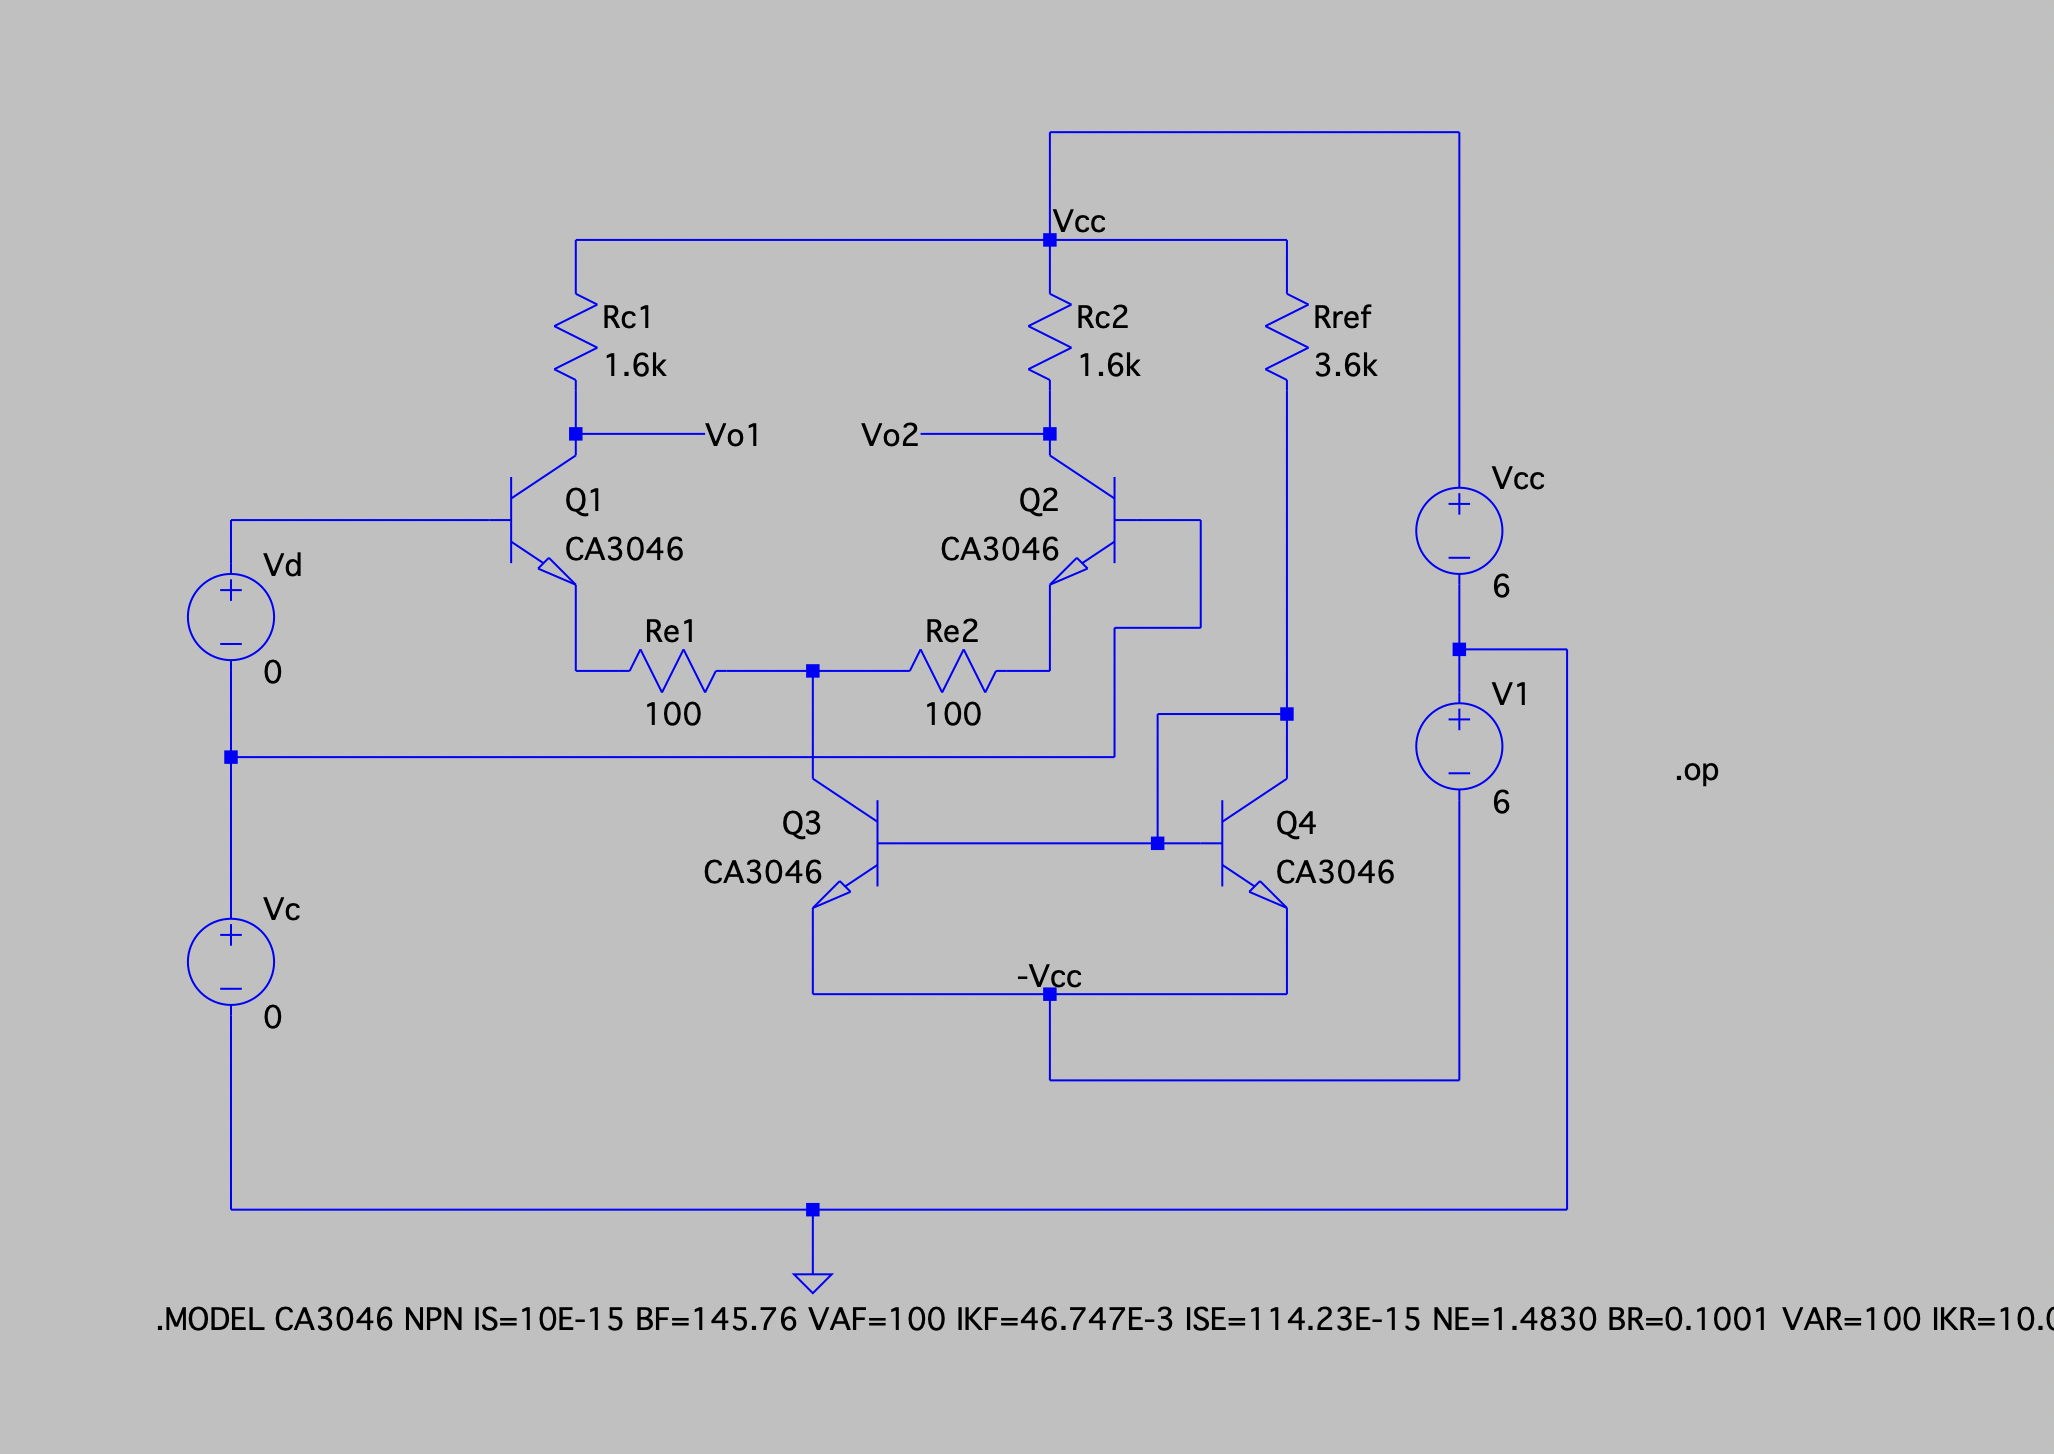
\includegraphics[scale=0.15\textscale]{scheme.png}
					    \captionof{figure}{Circuito Simulado em LTSpice}

                                  \end{minipage}
                          \end{figure}
	 \section{Questão 4.2}
	 	\begin{figure}[H]
			\centering
			\captionsetup{justification=centering}
			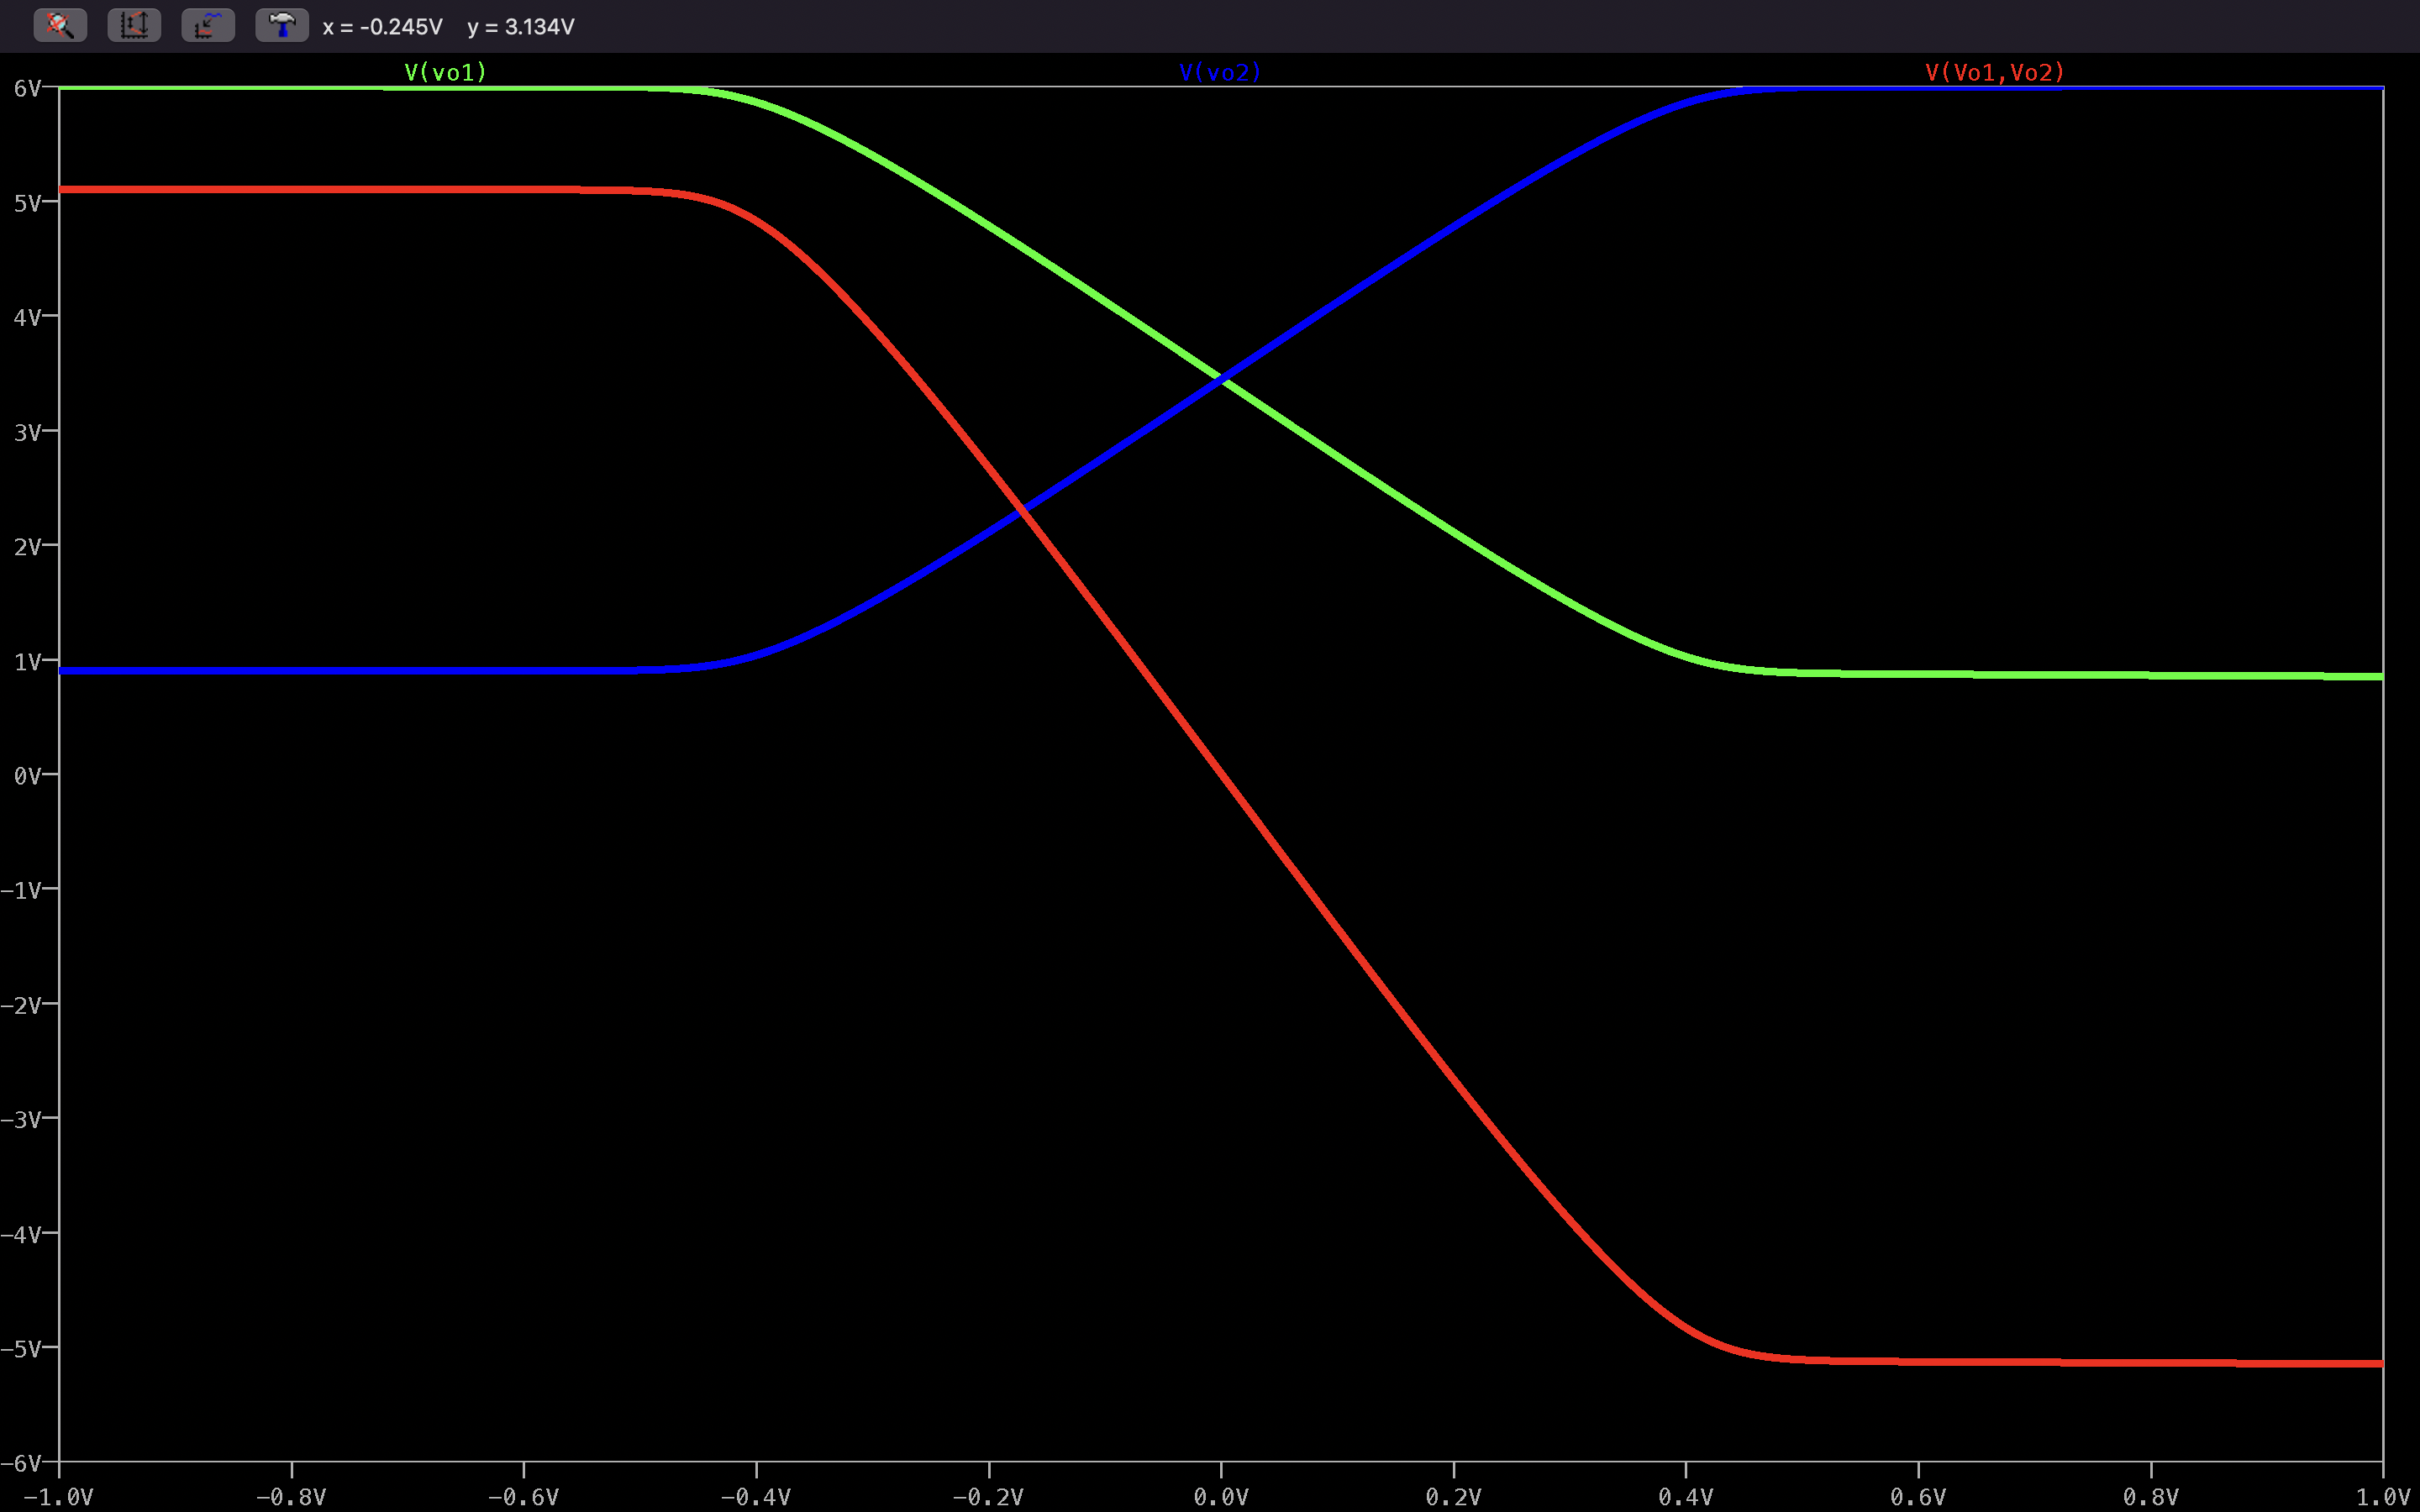
\includegraphics[scale=0.15\textscale]{4.2.png}
			\caption{}
		\end{figure}
	 \section{Questão 4.3}
	 \begin{figure}[H]
			\centering
			\captionsetup{justification=centering}
			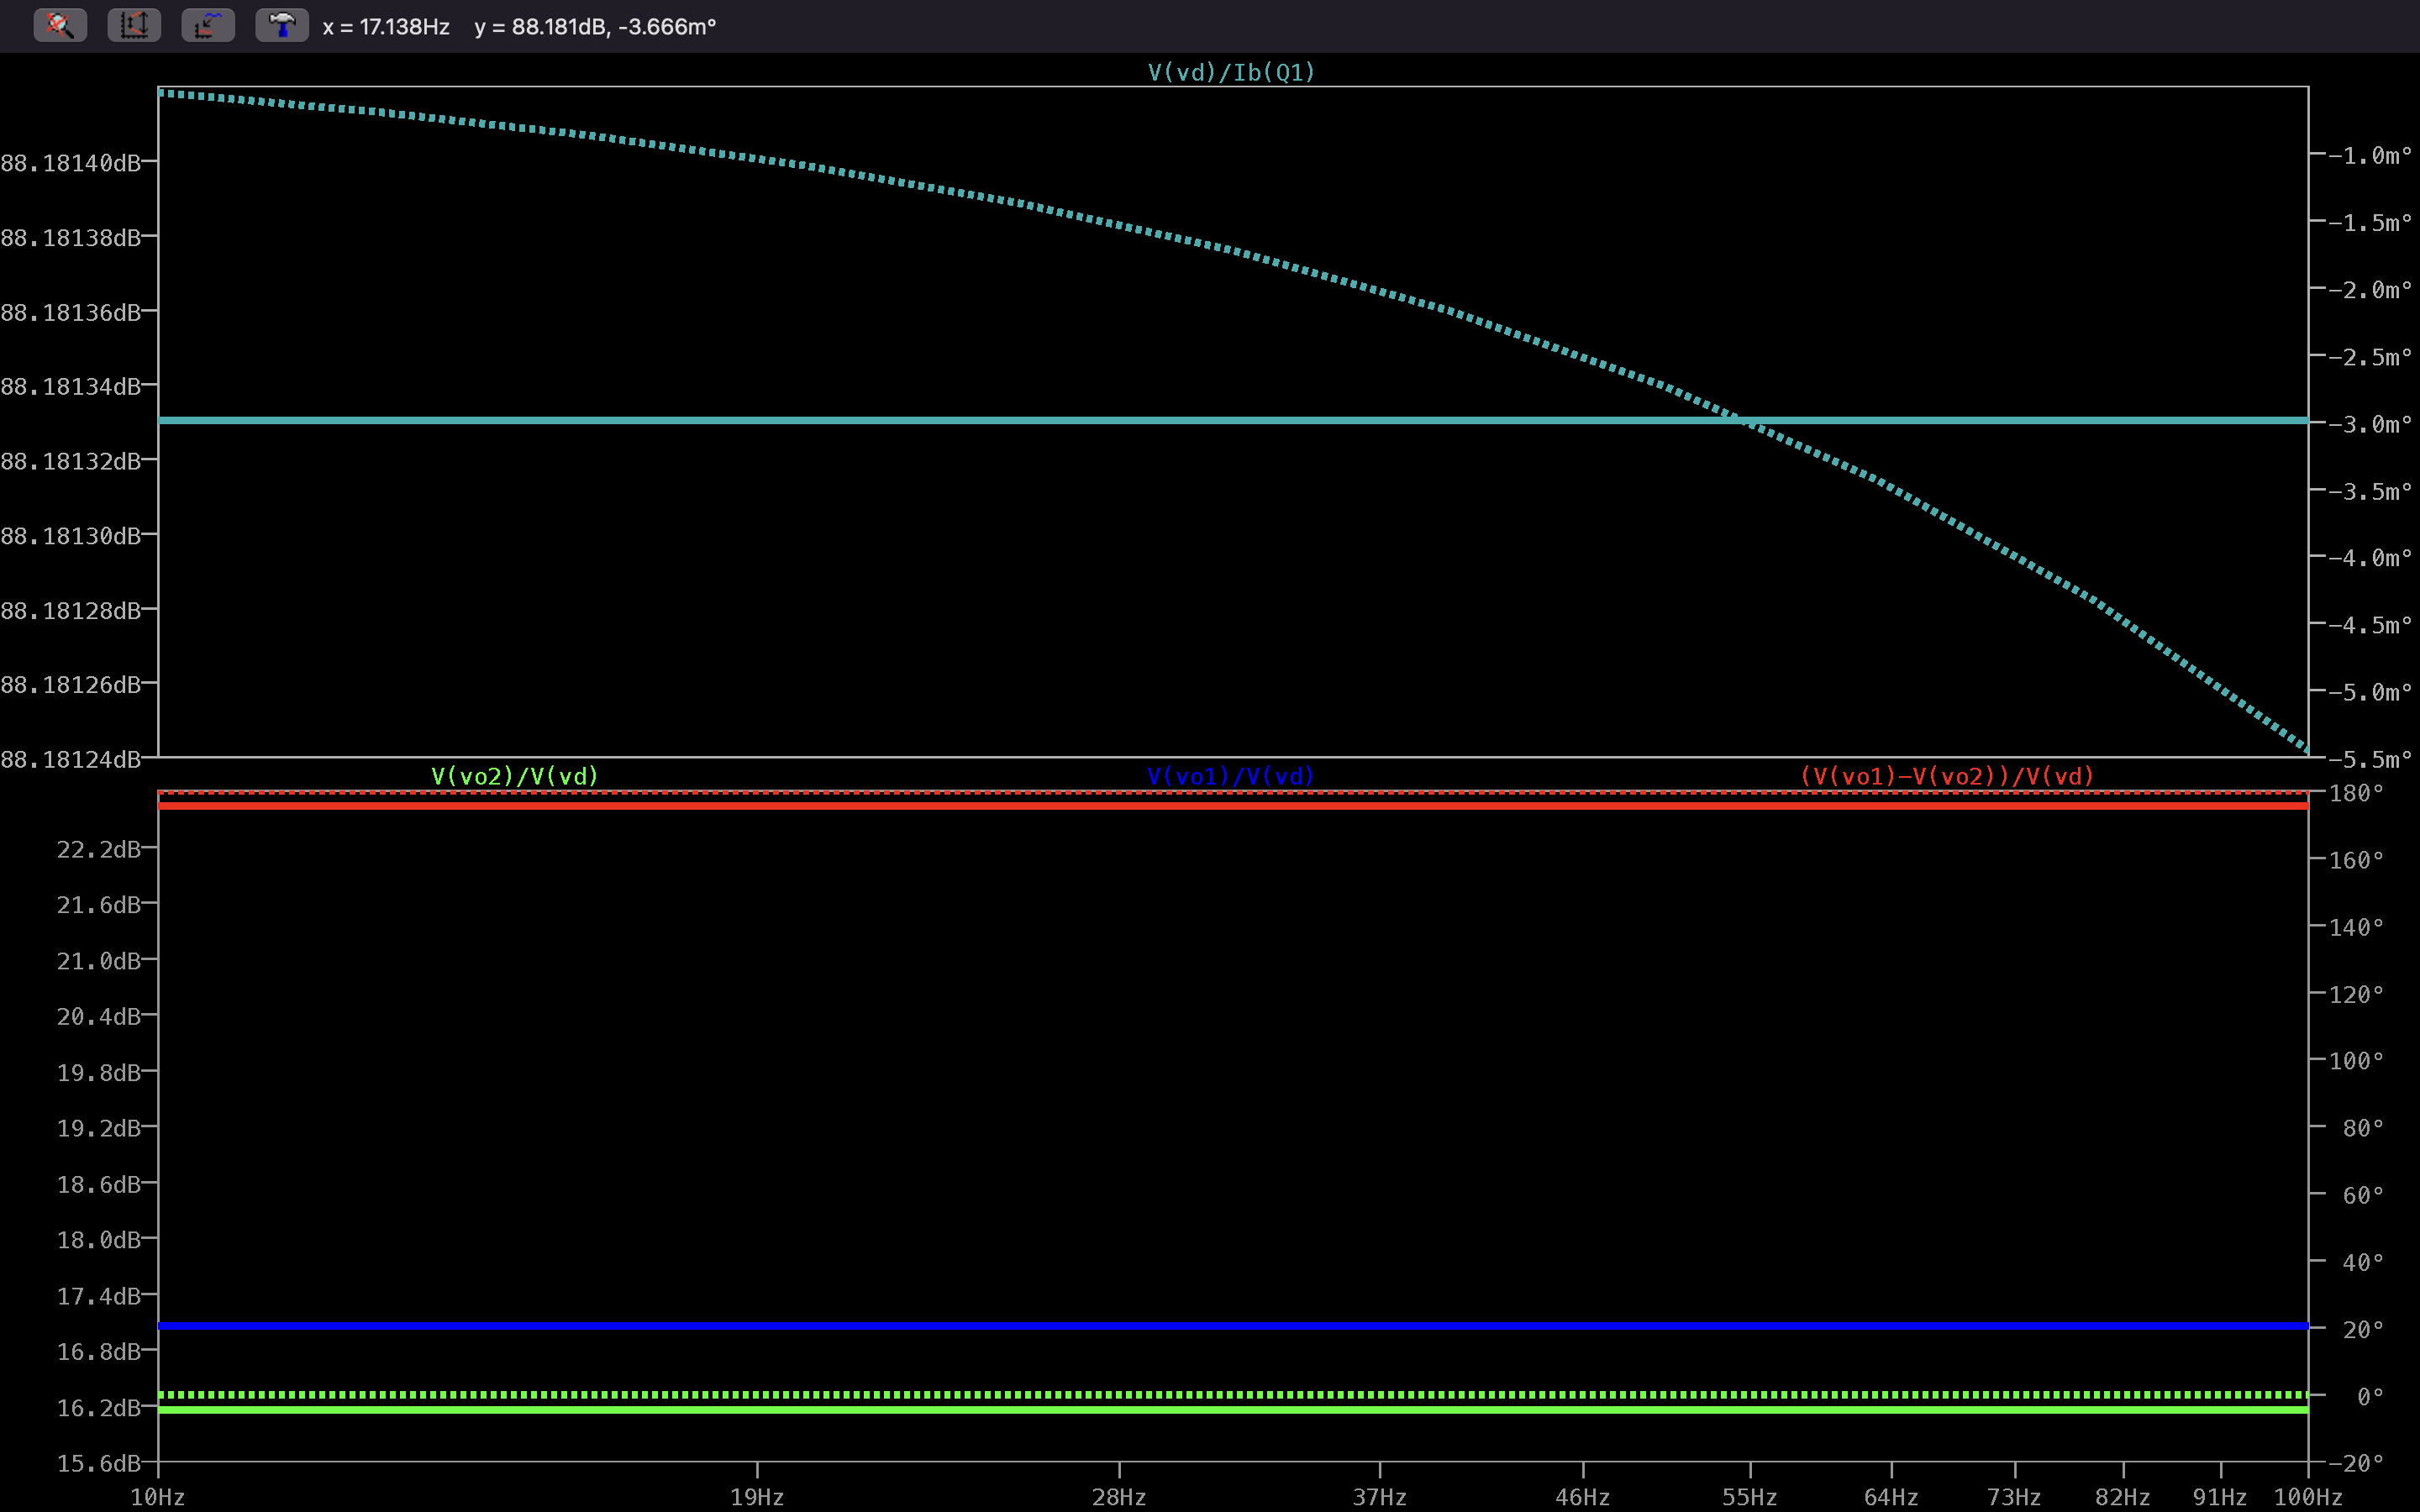
\includegraphics[scale=0.15\textscale]{4.3.png}
			\caption{}
		\end{figure}

         \section{Questão 4.4}
	 \begin{figure}[H]
			\centering
			\captionsetup{justification=centering}
			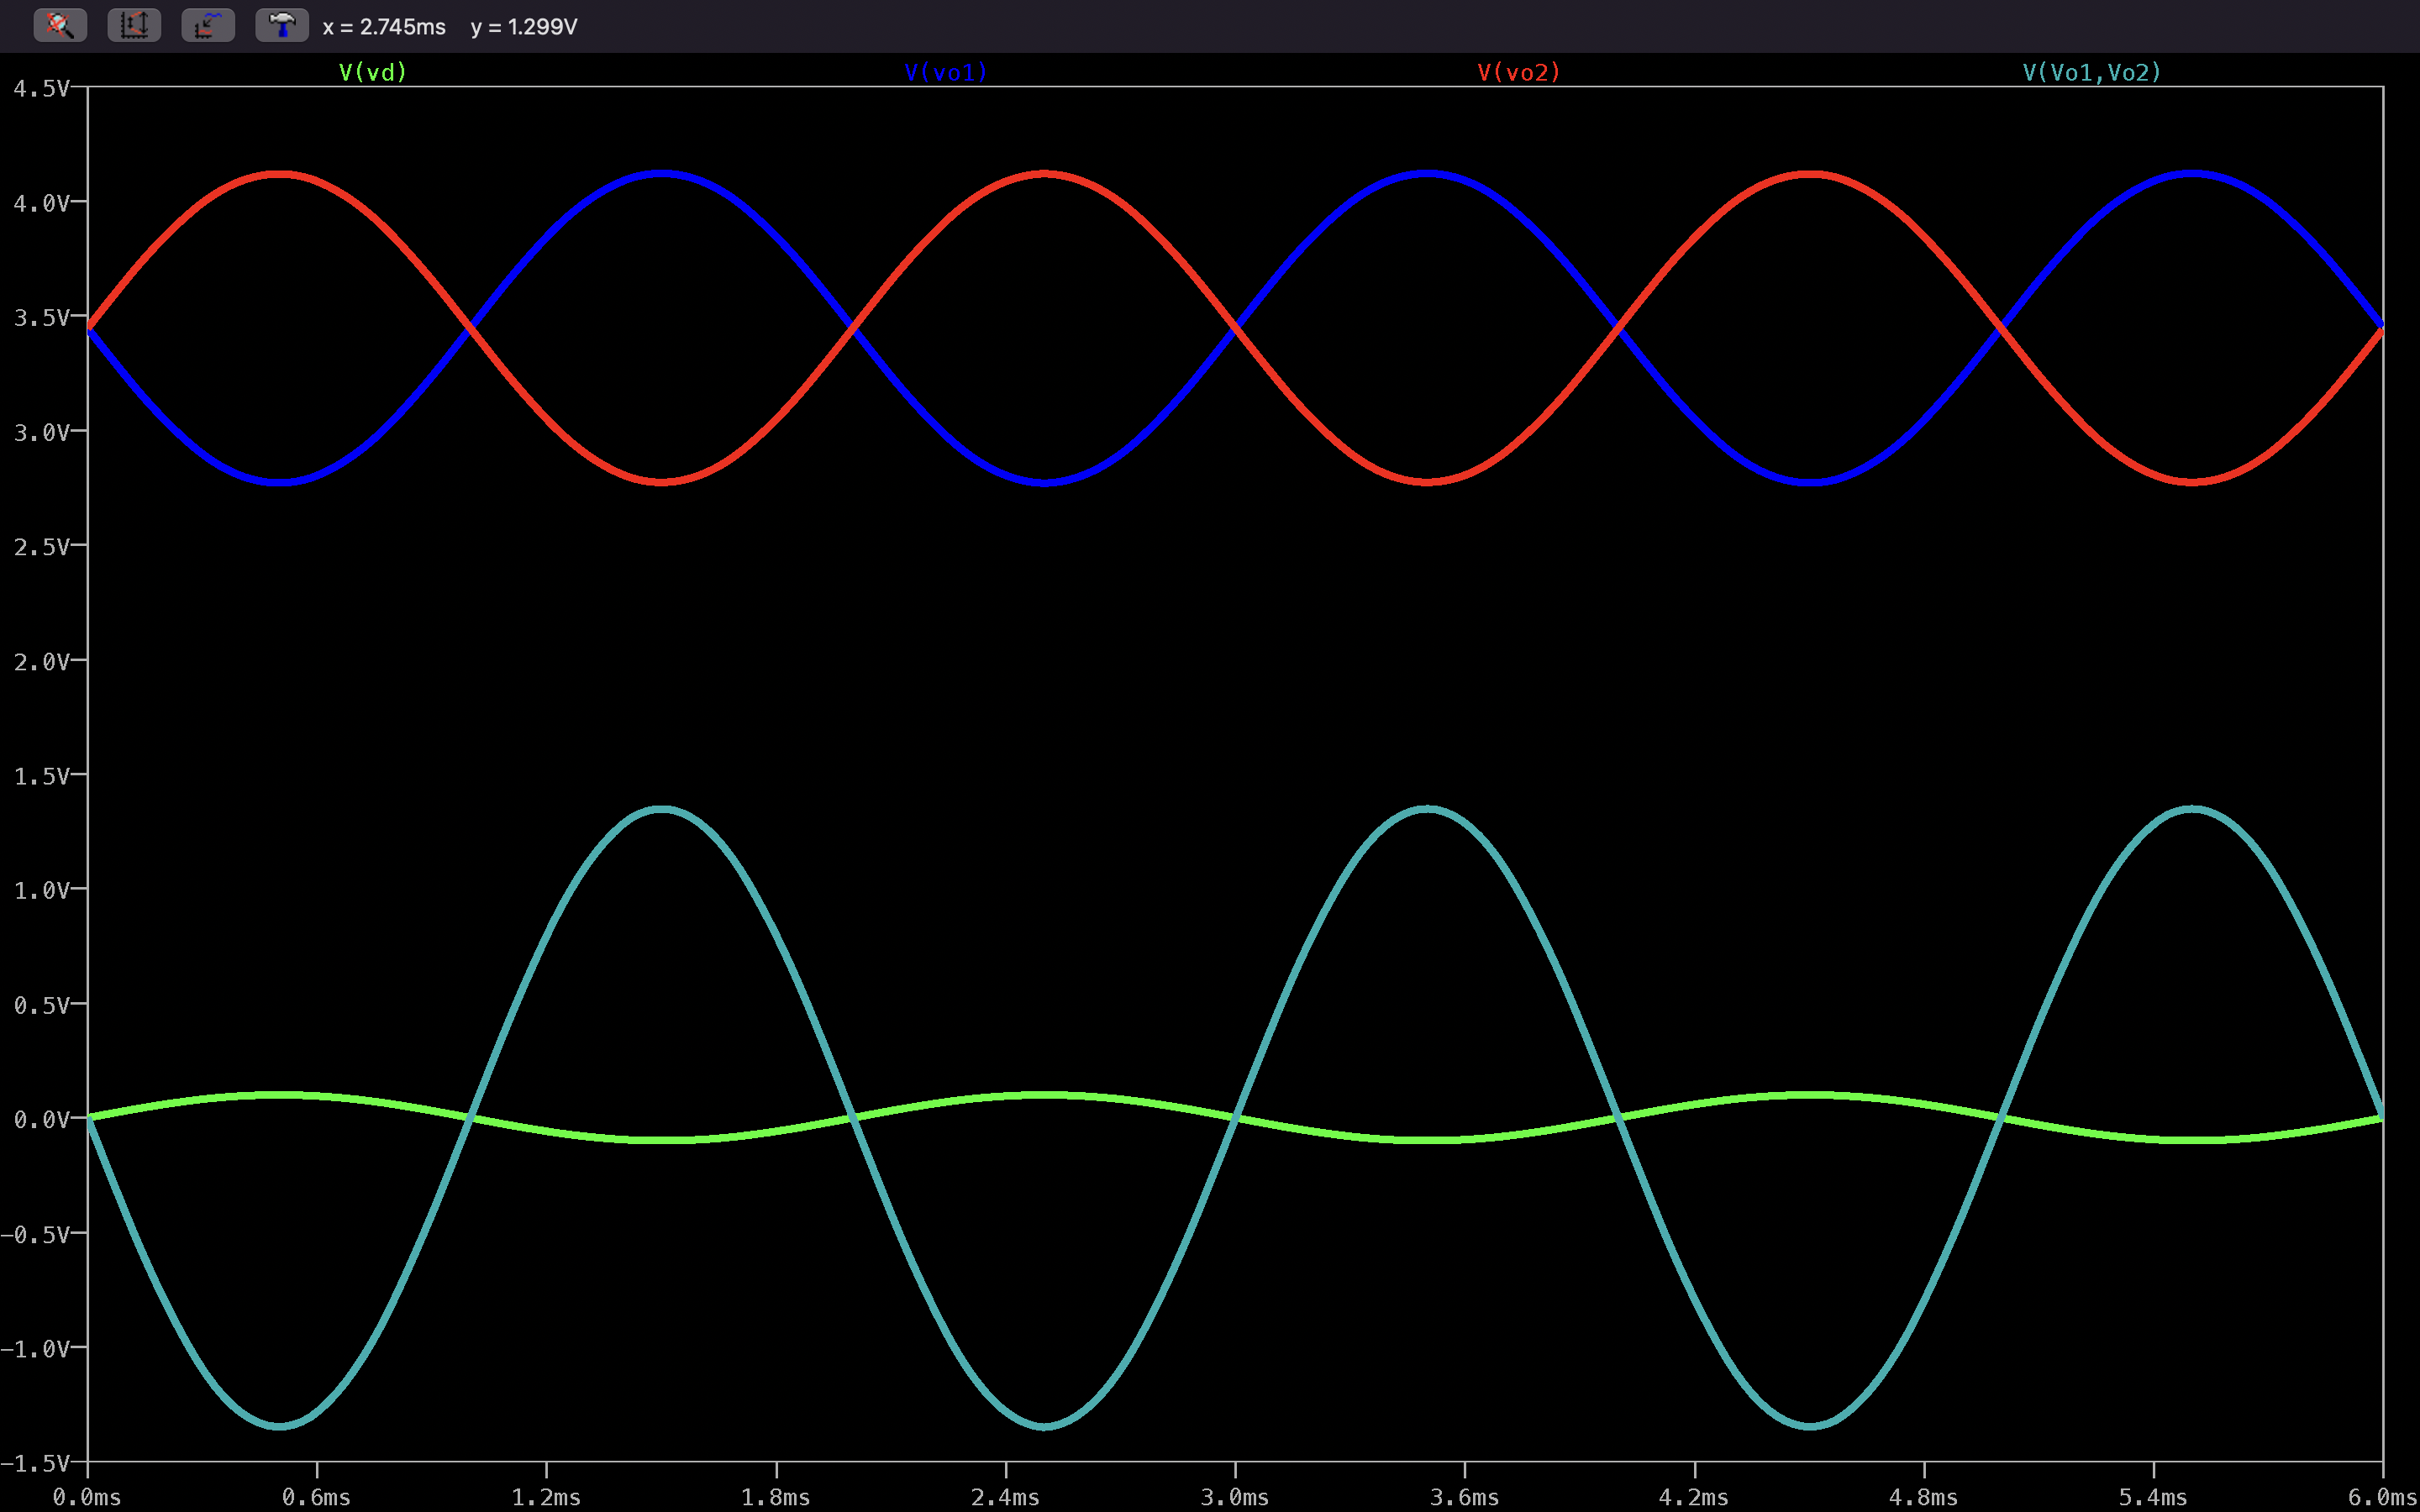
\includegraphics[scale=0.15\textscale]{4.4.png}
			\caption{}
		\end{figure}

	 \section{Questão 4.5}
	 \begin{figure}[H]
			\centering
			\captionsetup{justification=centering}
			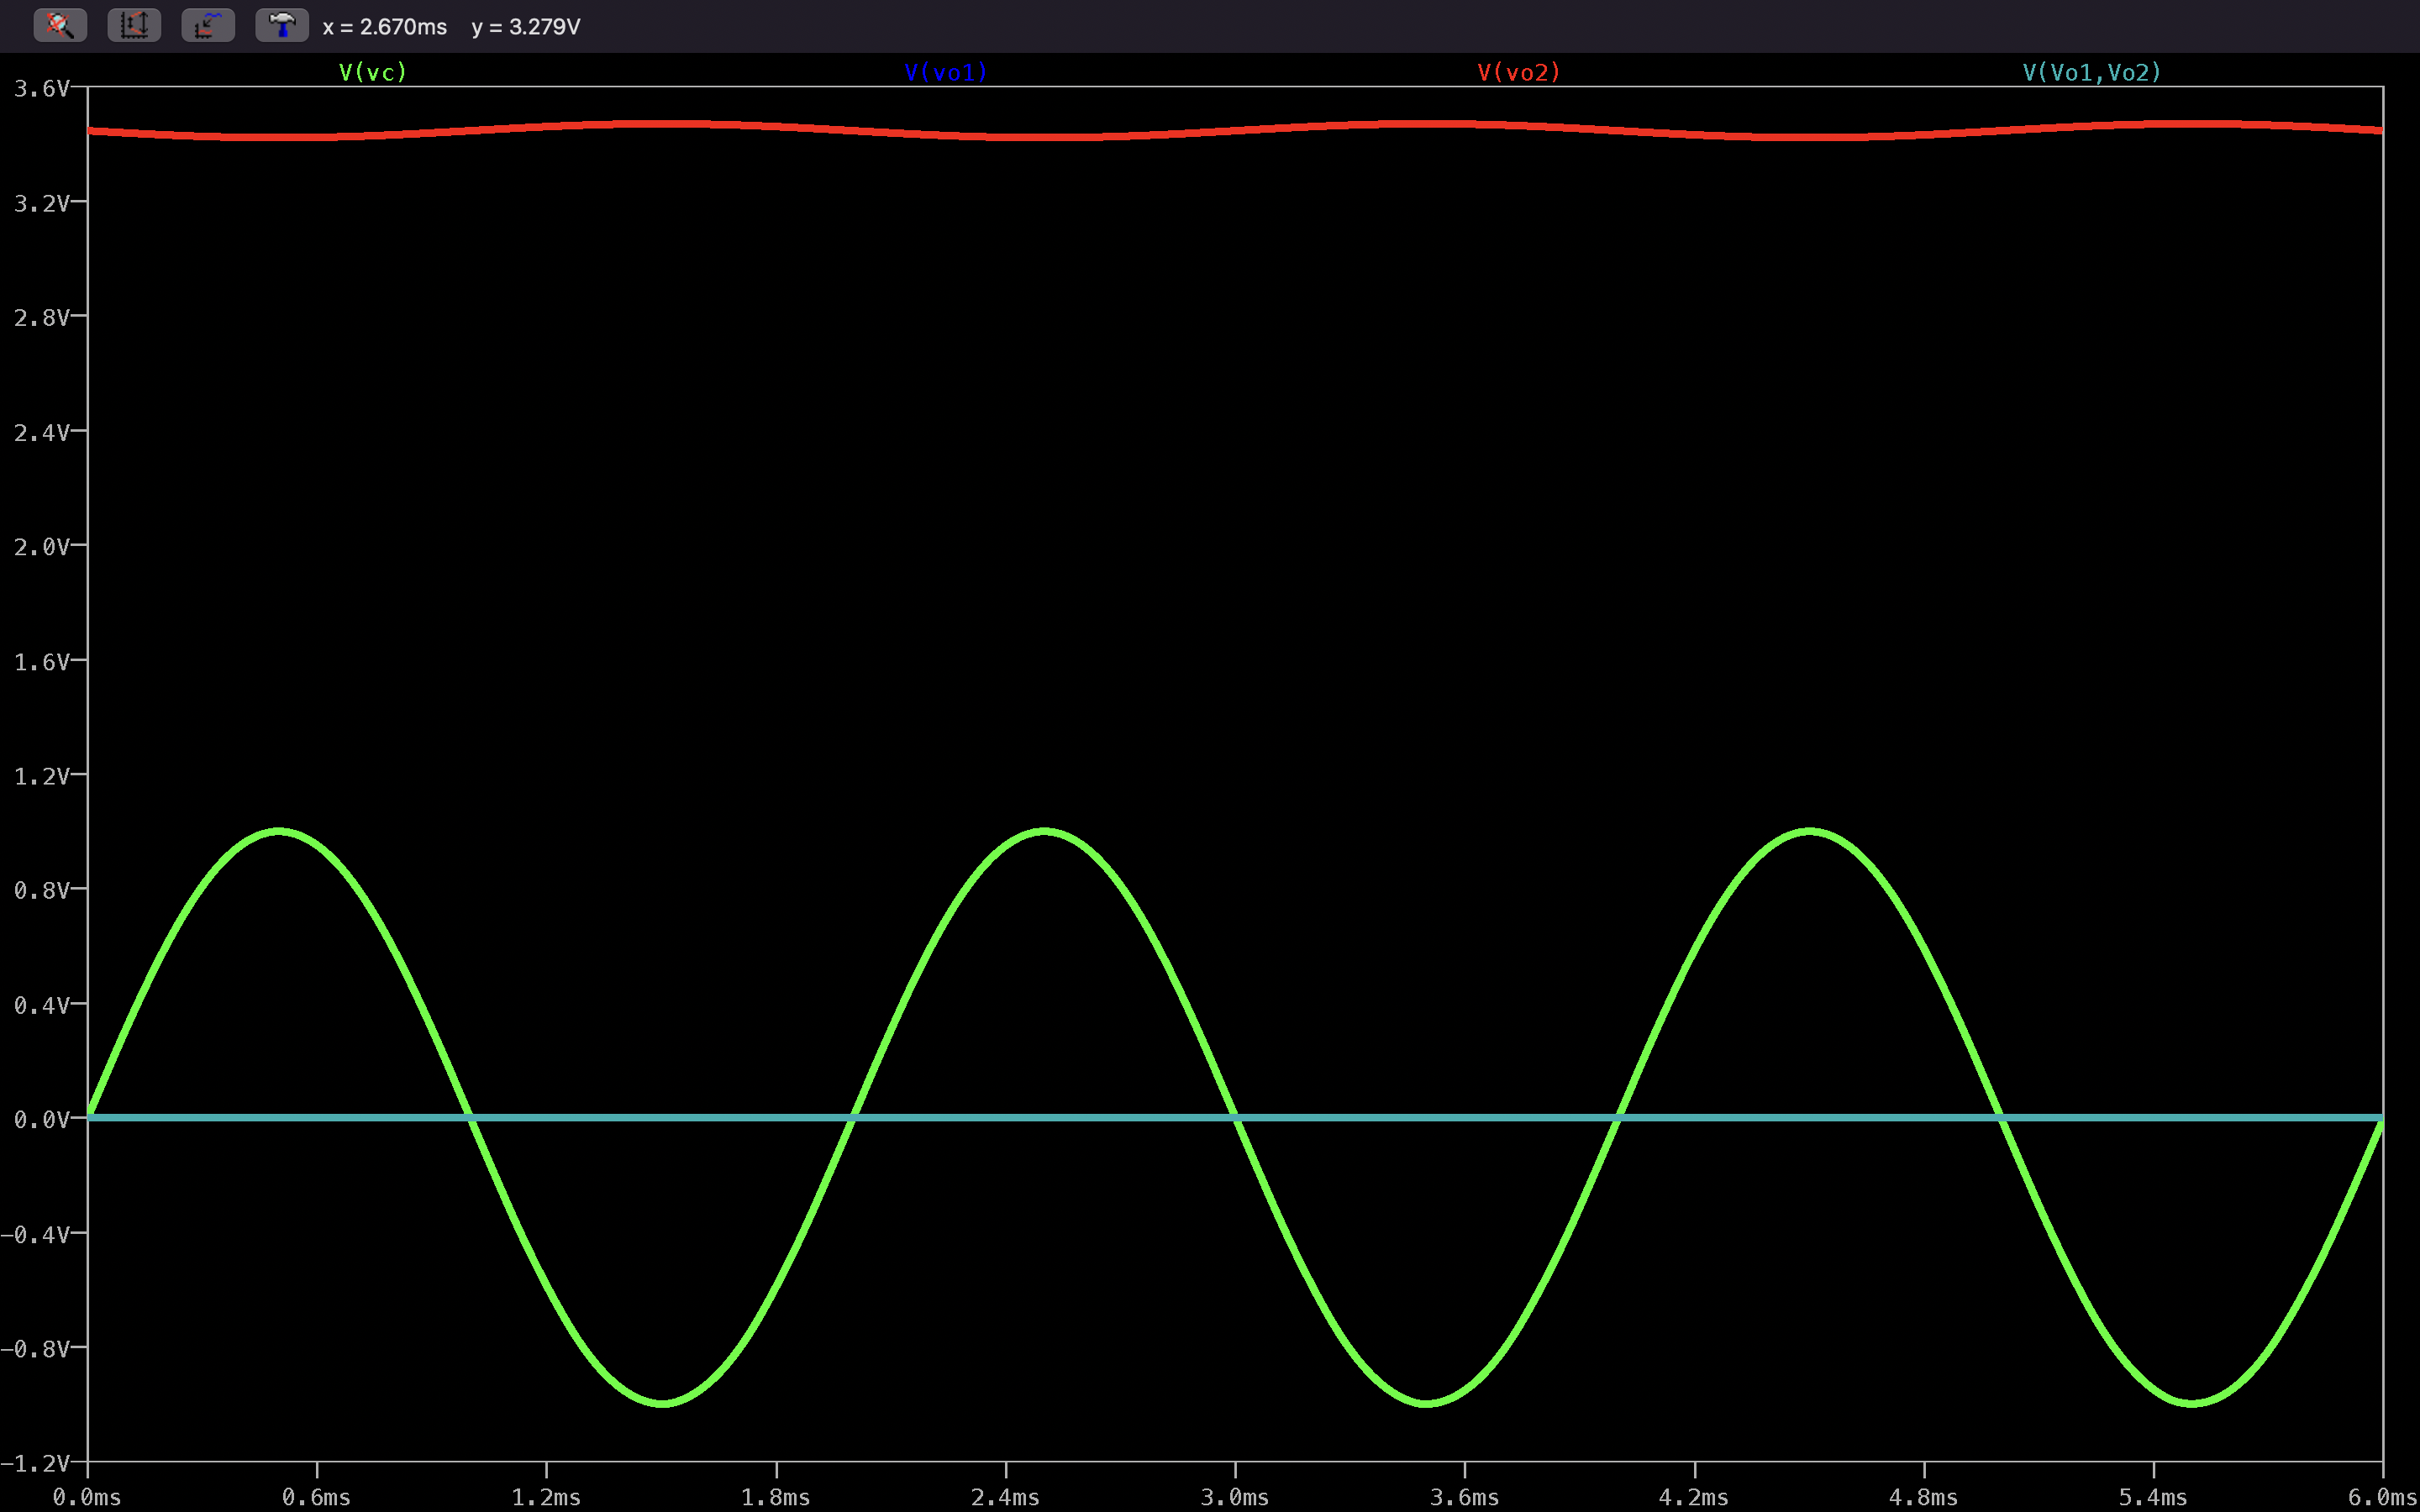
\includegraphics[scale=0.15\textscale]{4.5.png}
			\caption{}
		\end{figure}


	 \section{Questão 4.6}
	 \begin{figure}[H]
                          \centering
                          \captionsetup{justification=centering}
                          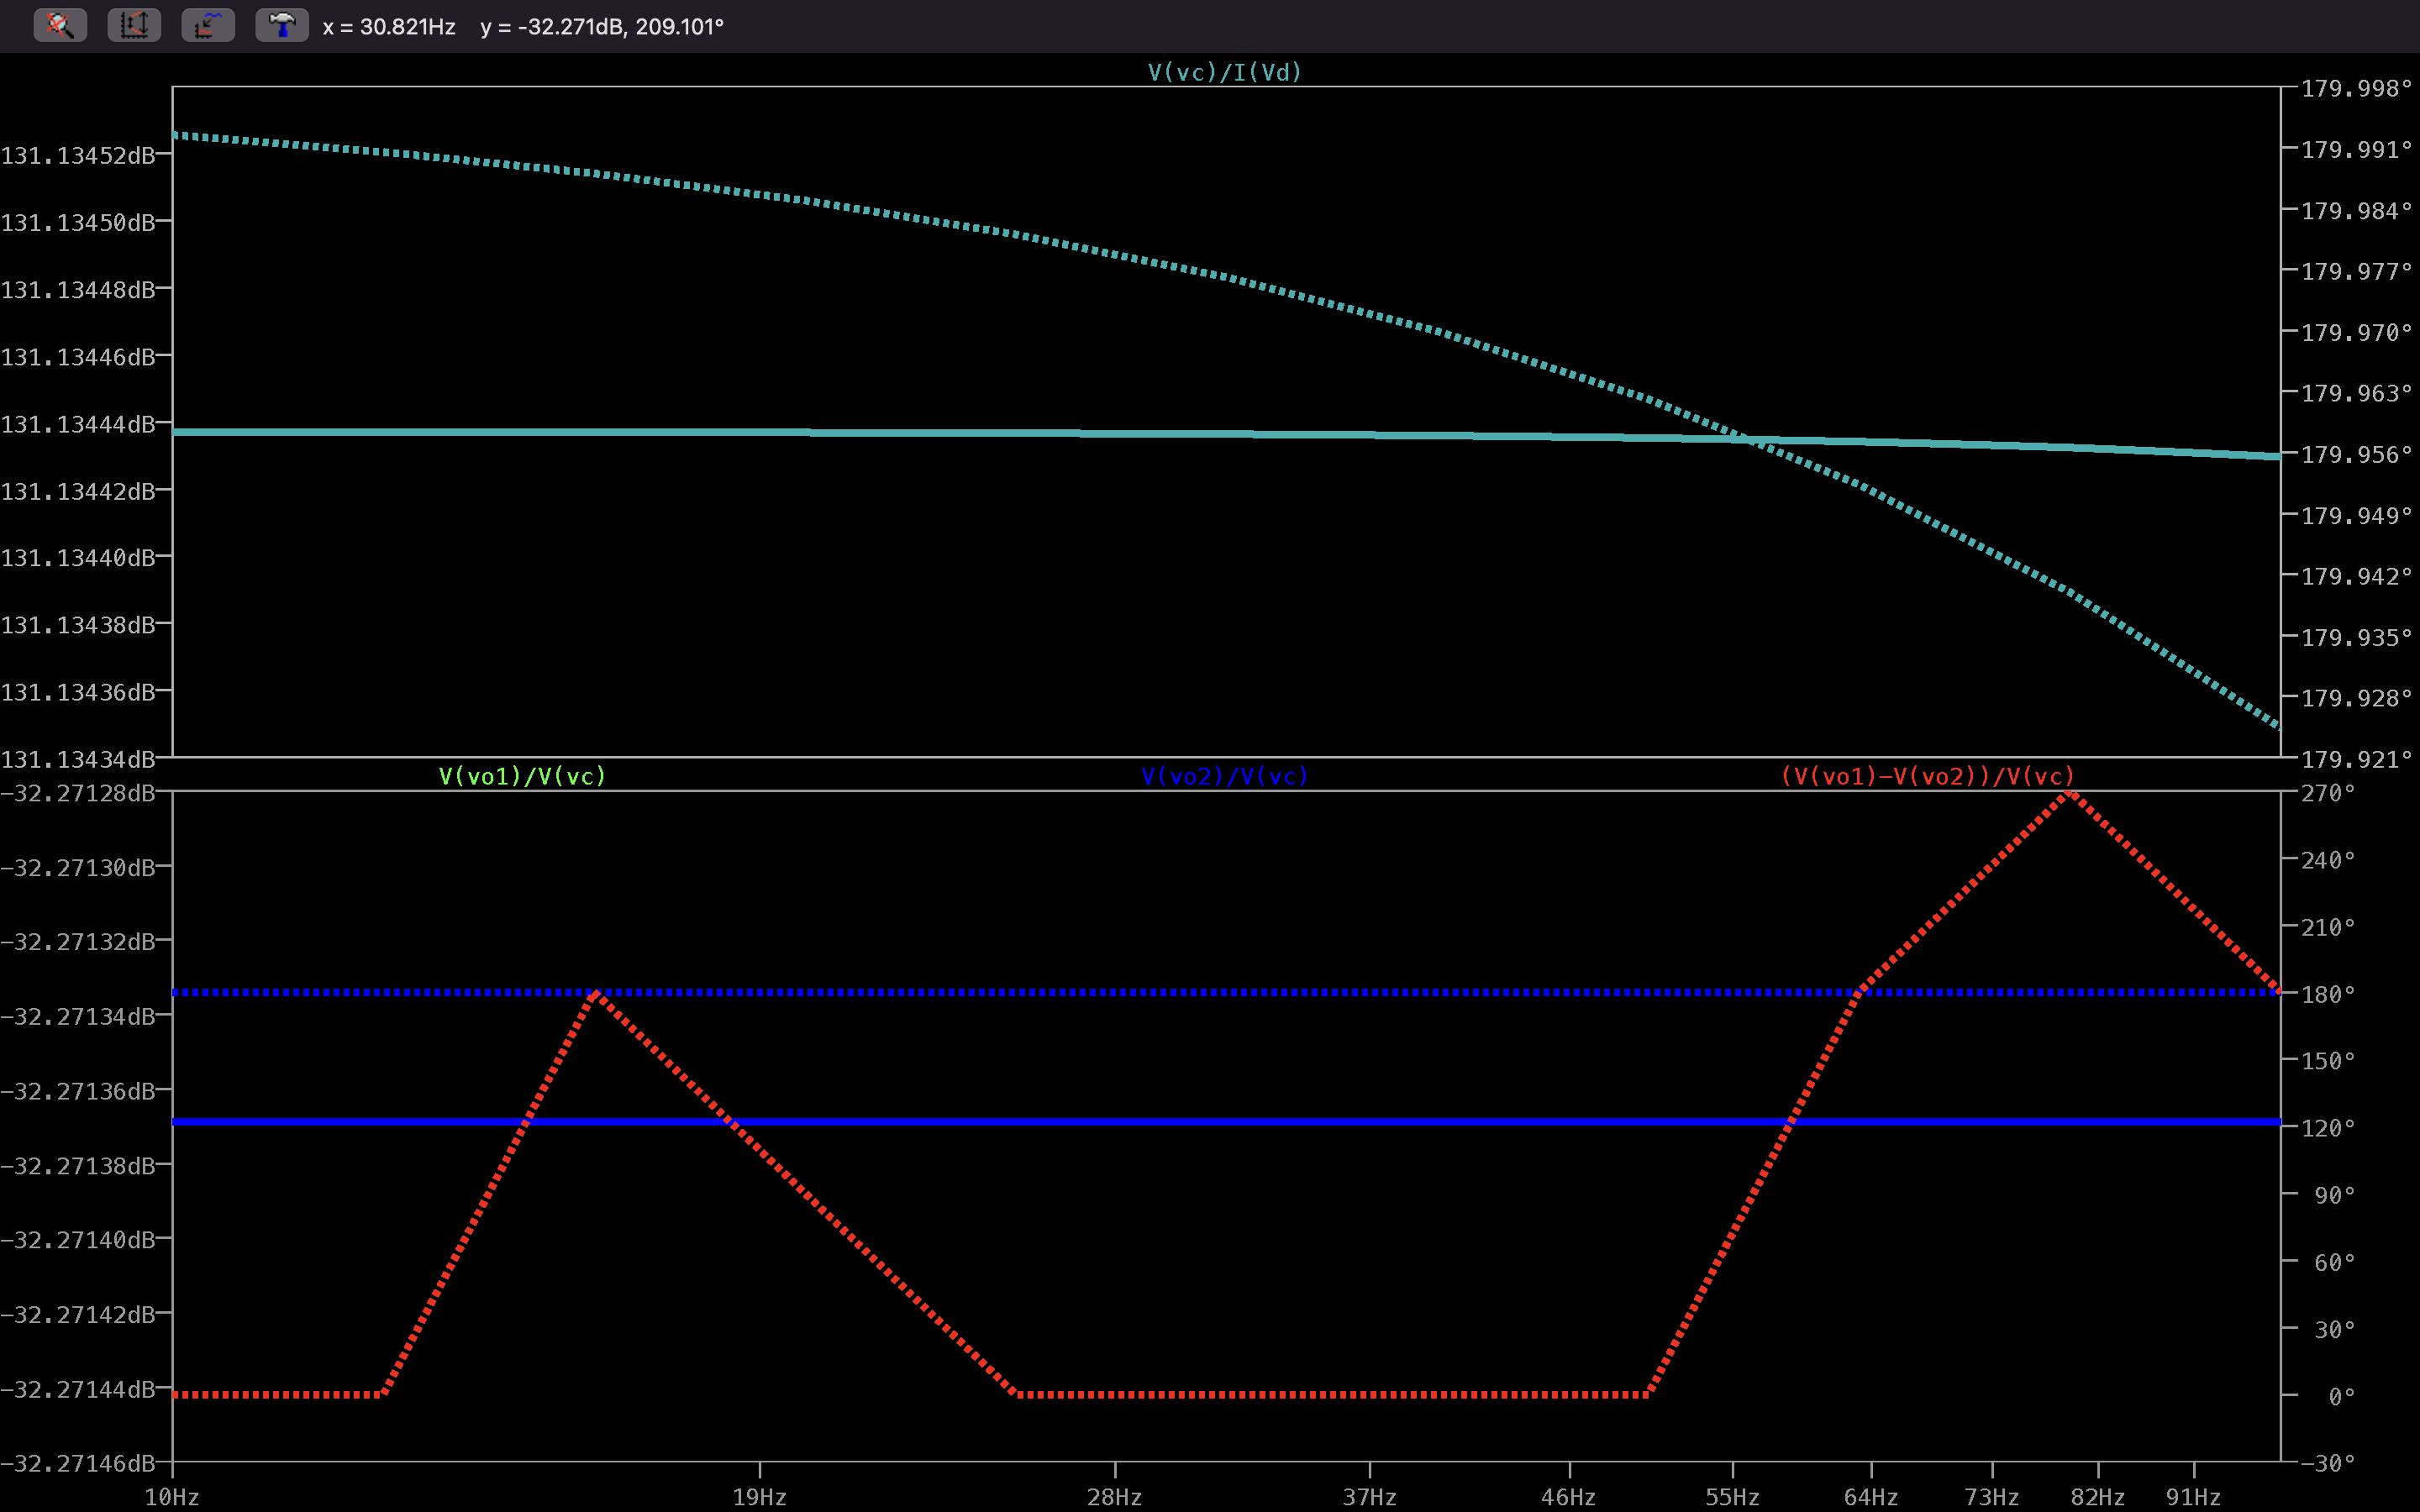
\includegraphics[scale=0.15\textscale]{4.6.png}
                          \caption{}
                  \end{figure}
	 \section{Questão 4.7}
		\begin{figure}[H]
                            \centering
                            \captionsetup{justification=centering}
                            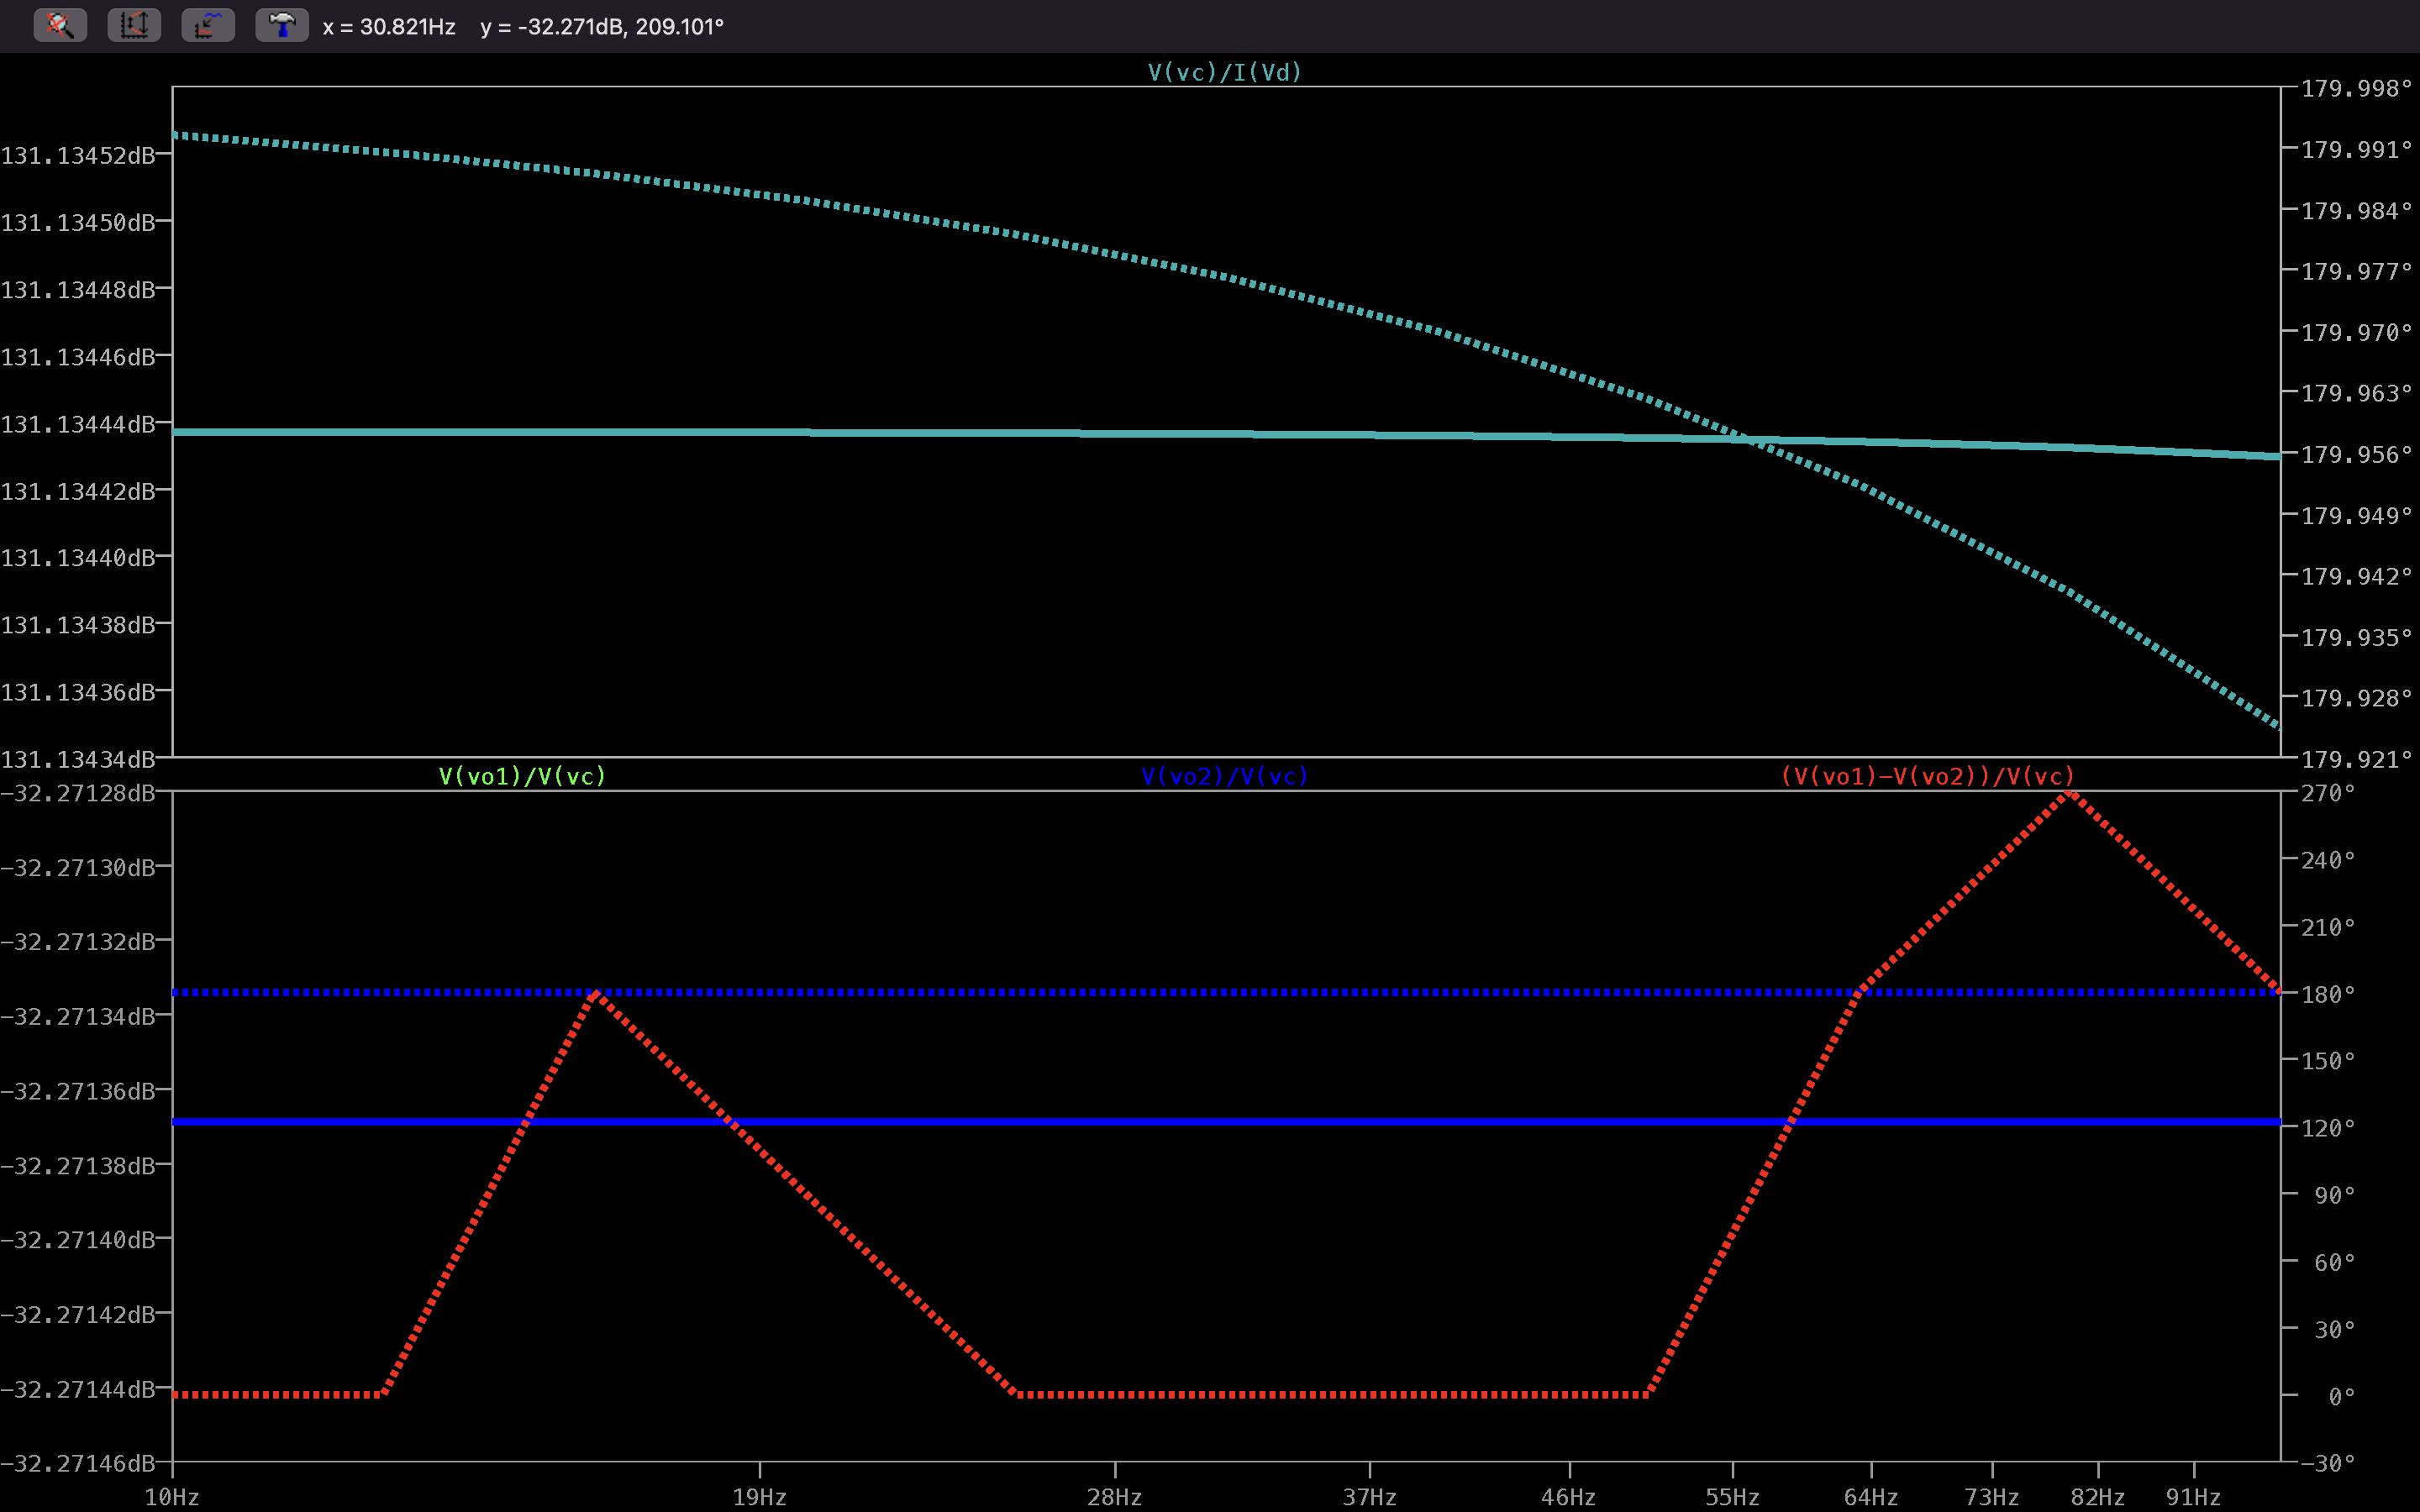
\includegraphics[scale=0.15\textscale]{4.6.png}
                            \caption{}
                    \end{figure}
		    \begin{center}
			    \begin{equation}
				    CMRR=\frac{22.6}{0}=\infty
				\end{equation}
			\begin{equation}
				CMRR1=\frac{10^{\frac{17}{20}}}{10^{\frac{-32}{20}}}=28
			\end{equation}
		\end{center}
	 \section{Questão 4.8}
	 	\begin{figure}[H]
                            \centering
                            \captionsetup{justification=centering}
                            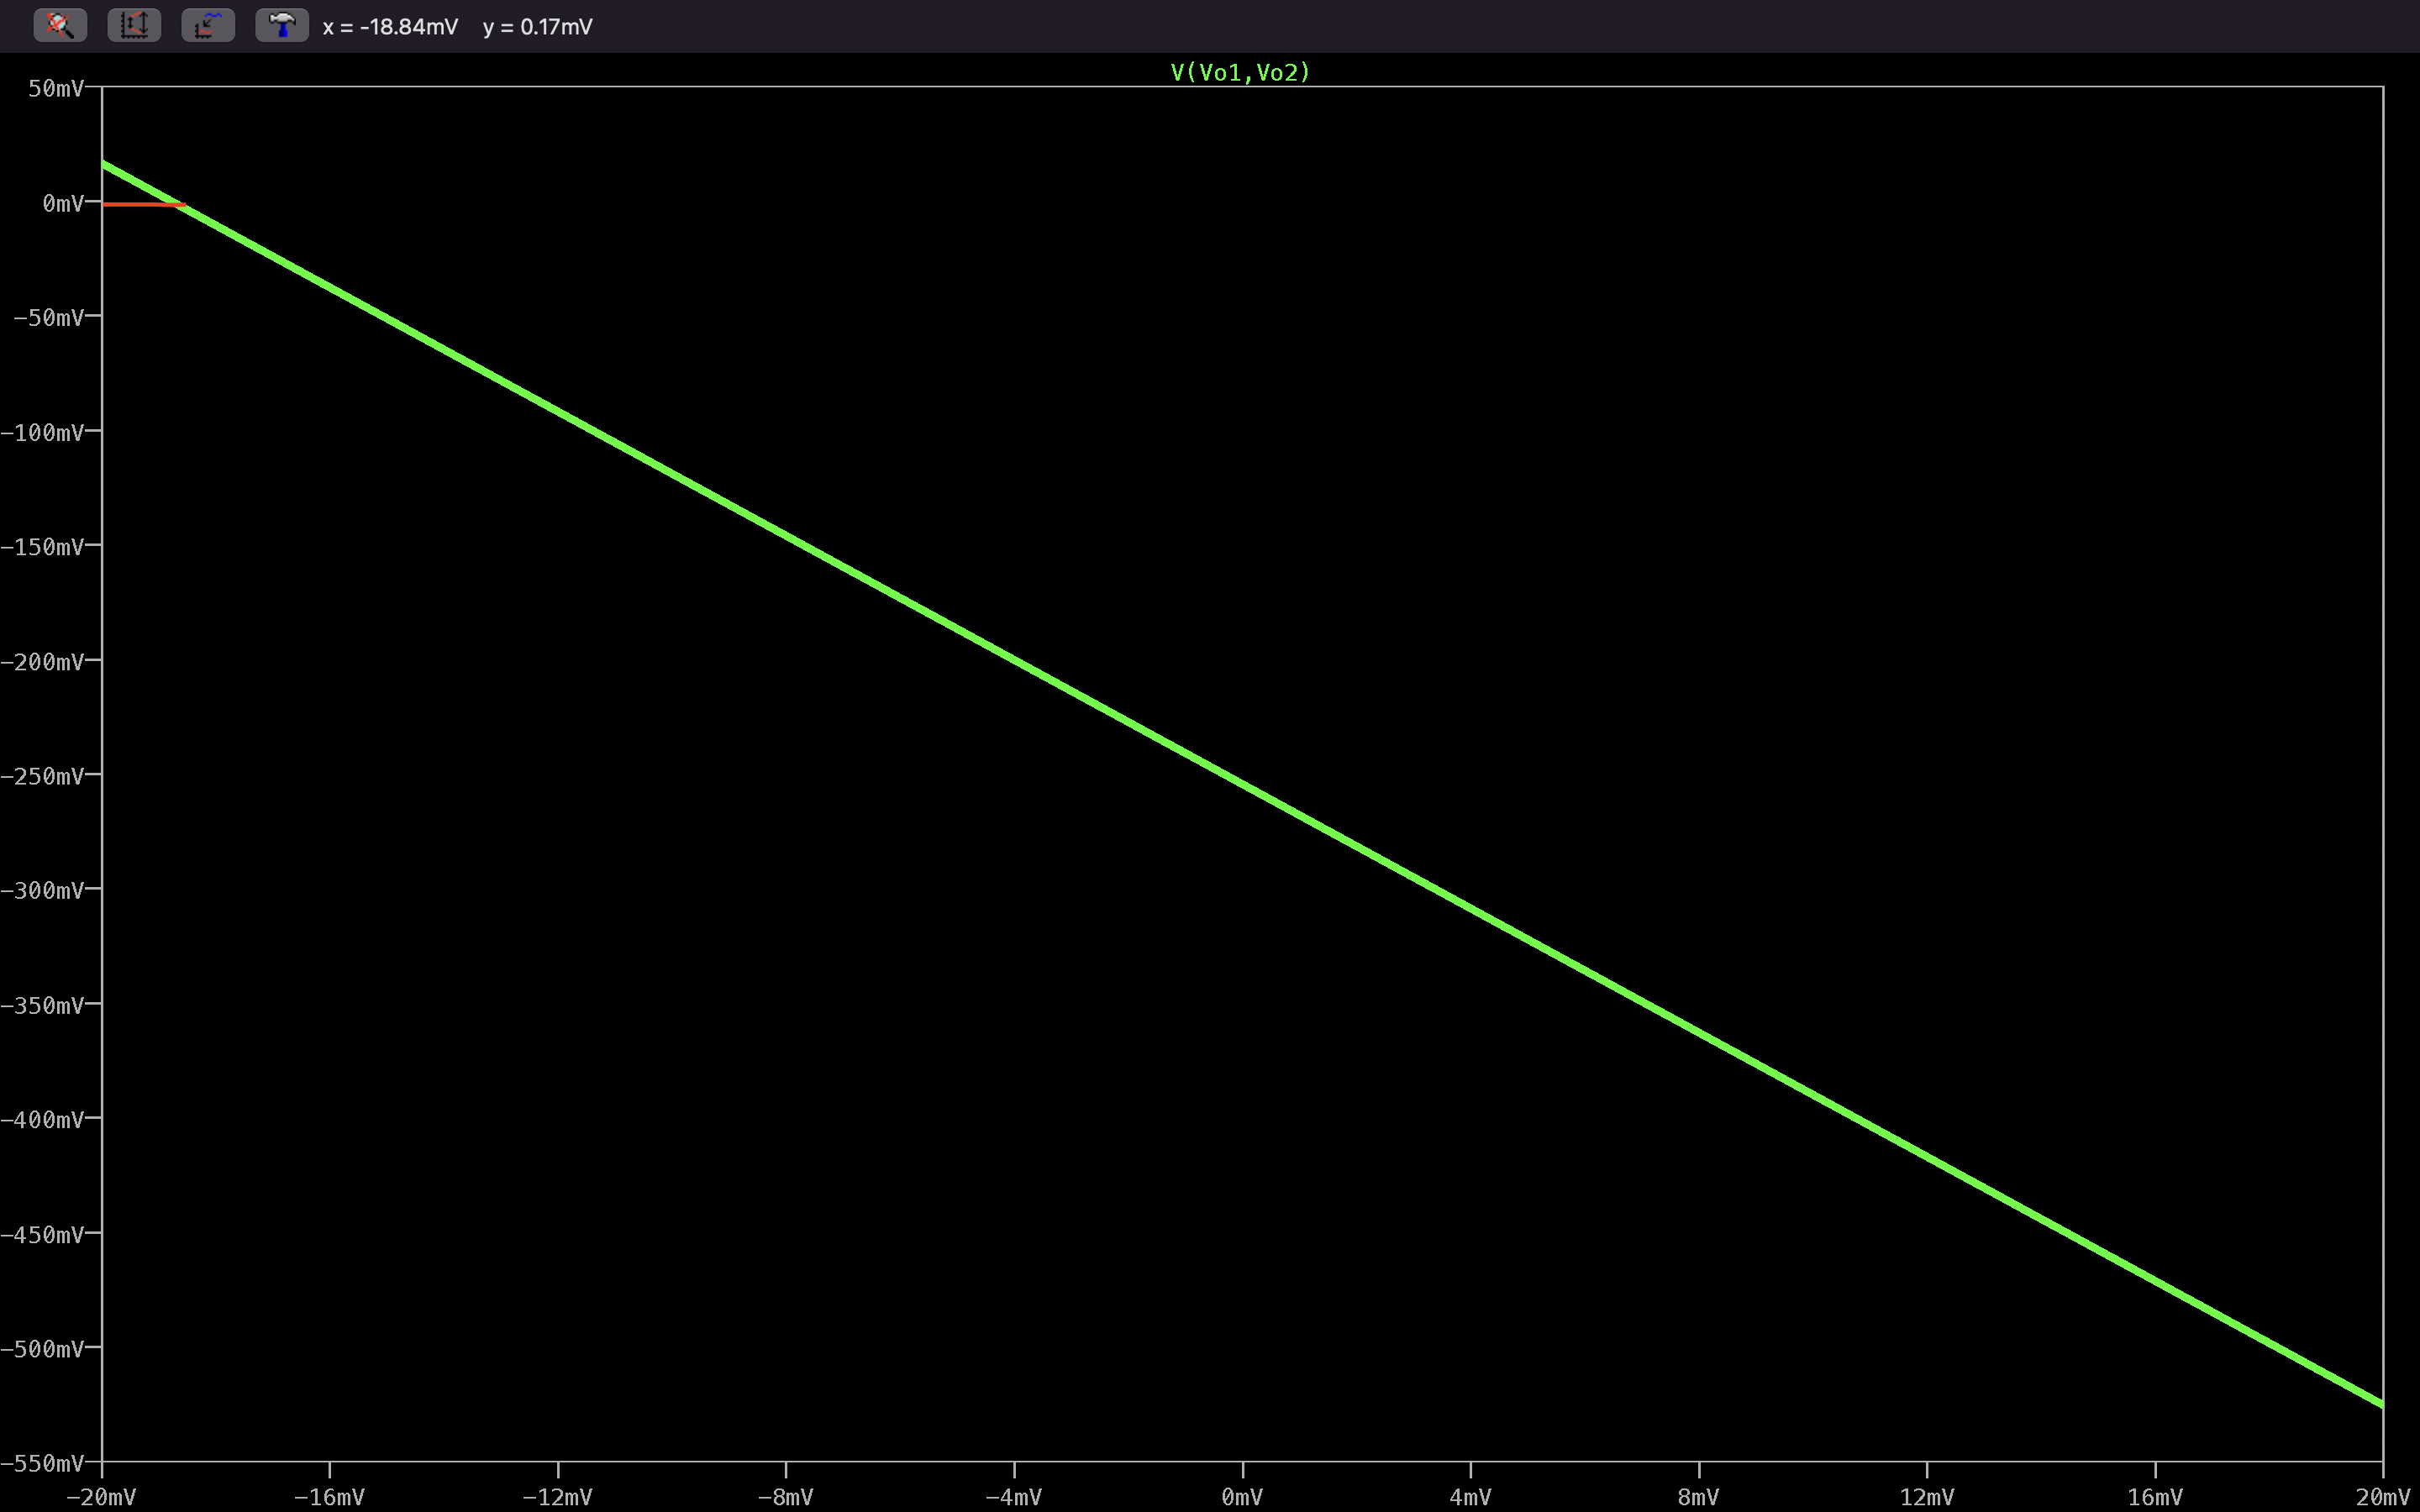
\includegraphics[scale=0.15\textscale]{4.8.png}
                            \caption{}
                    \end{figure}
	\newpage 
	\section{Questão 5.1}
	 \begin{figure}[h]
		 \centering
		\begin{minipage}[c]{0.2 \textwidth}
	 		\begin{table}[H]
				\captionsetup{justification=centering}
						 \begin{tabular}{|c||c|}	
					\hline
						V$_{CC}$  & 5.97 V \\ \hline
						V$_{EE}$  & 5.91 V \\ \hline
						V$_{o1}$  & 3.34 V \\ \hline
						V$_{o2}$  & 3.36 V \\ \hline
						V$_{C4}$  & 4.99 V \\ \hline
						V$_{RE1}$ &0.161  V \\ \hline
						V$_{RE2}$ &0.163 V \\ \hline
				
				\end{tabular}
				\caption{Valores medidos experimentalmente}
			\end{table}
		\end{minipage}
		\hspace{0.1\textwidth}	
                                \begin{minipage}[T]{0.4\textwidth}
                                          \centering
                                          \captionsetup{justification=centering}
                                          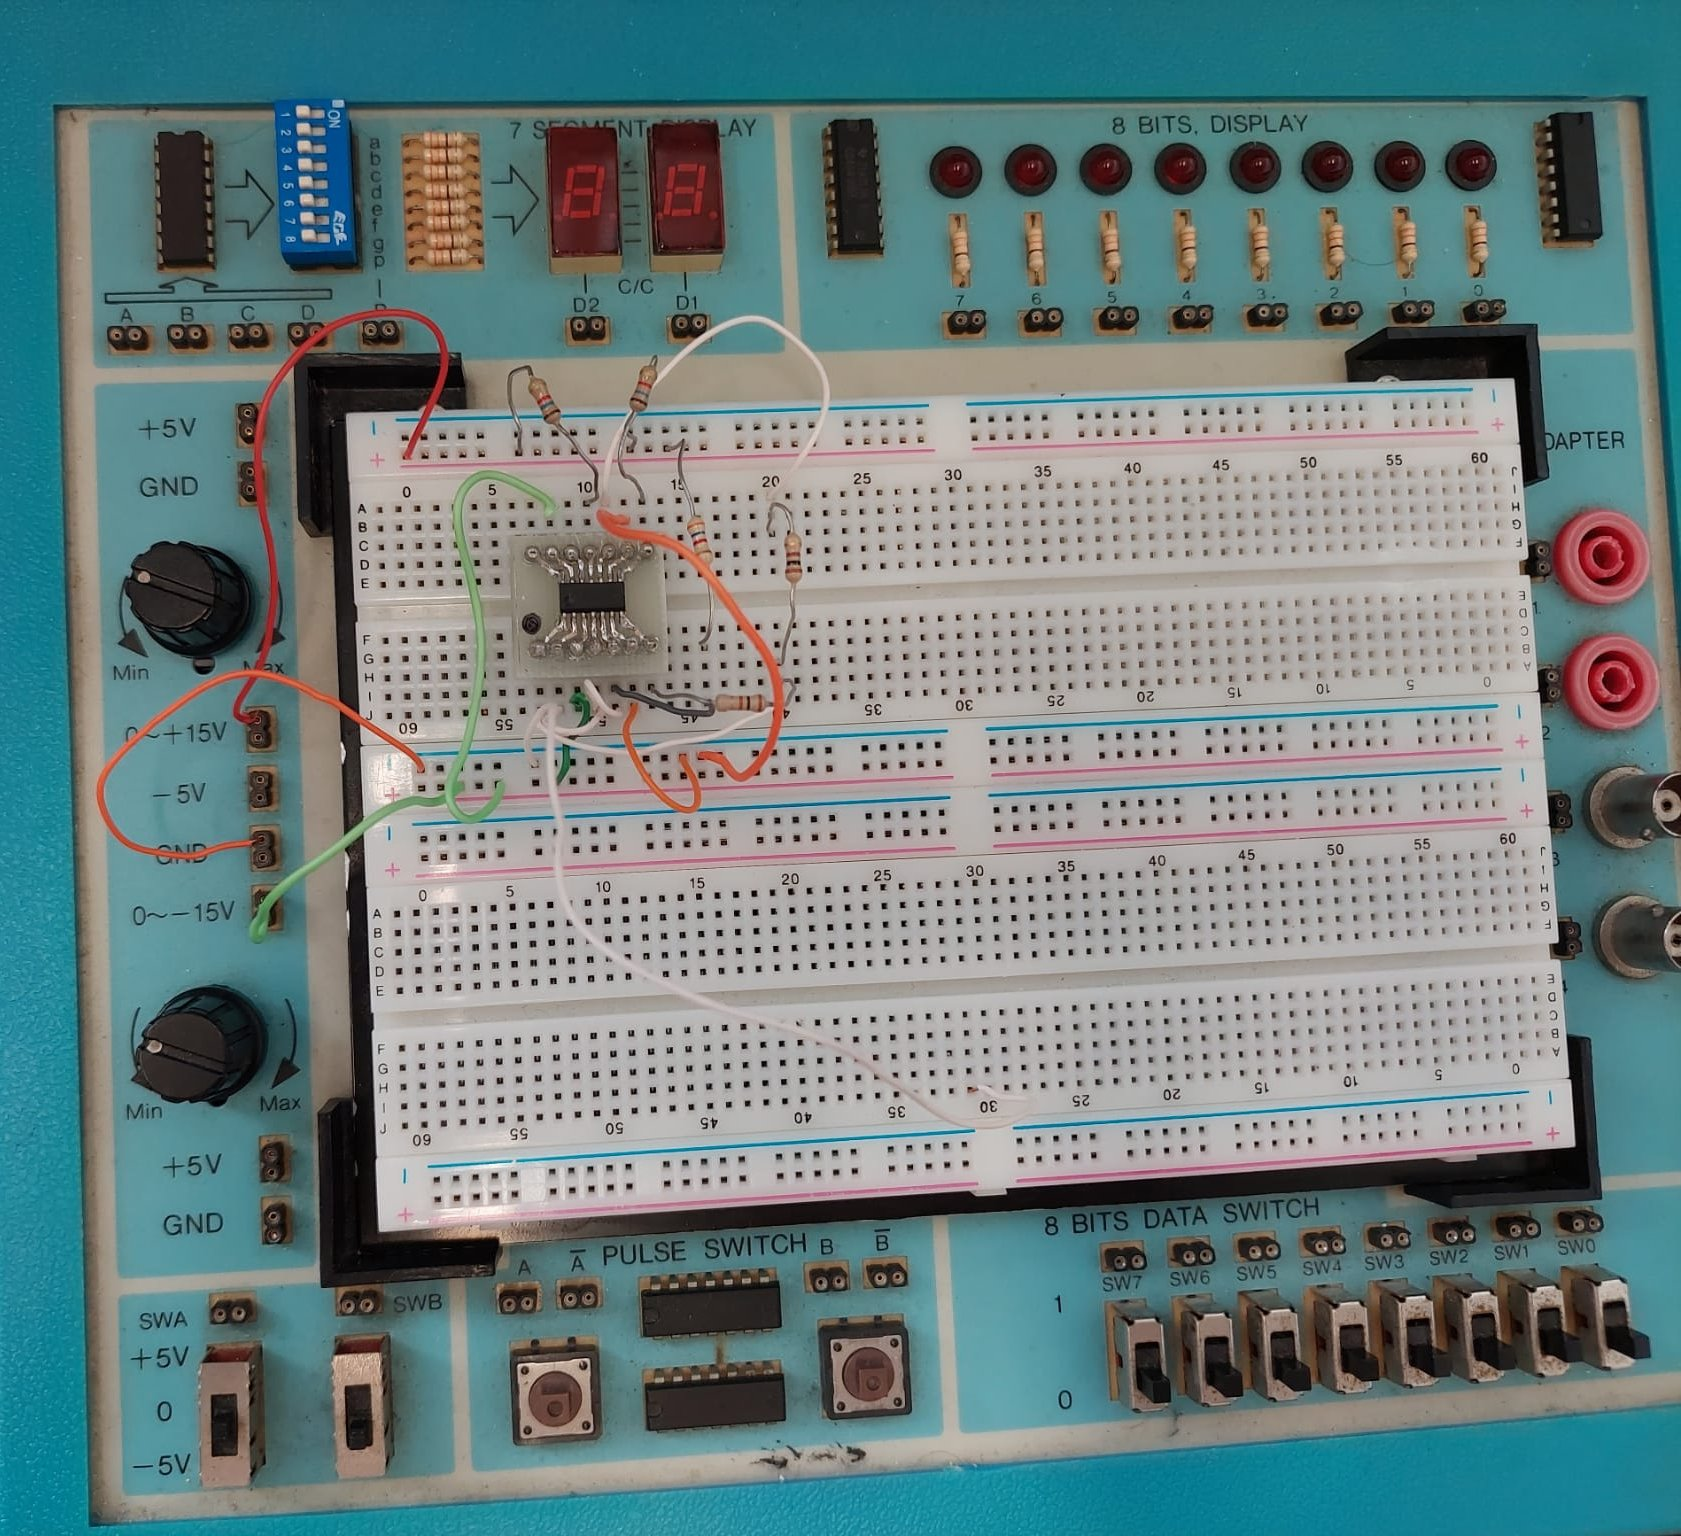
\includegraphics[scale=0.1\textscale]{assembly.jpg}
                                        \captionof{figure}{Montagem realizada em contexto laboratorial}

                                \end{minipage}
			\end{figure}
	\section{Questão 5.2}
		 \begin{figure}[H]
                                          \centering
                                          \begin{minipage}{0.45\textwidth}
                                                  \centering
                                                  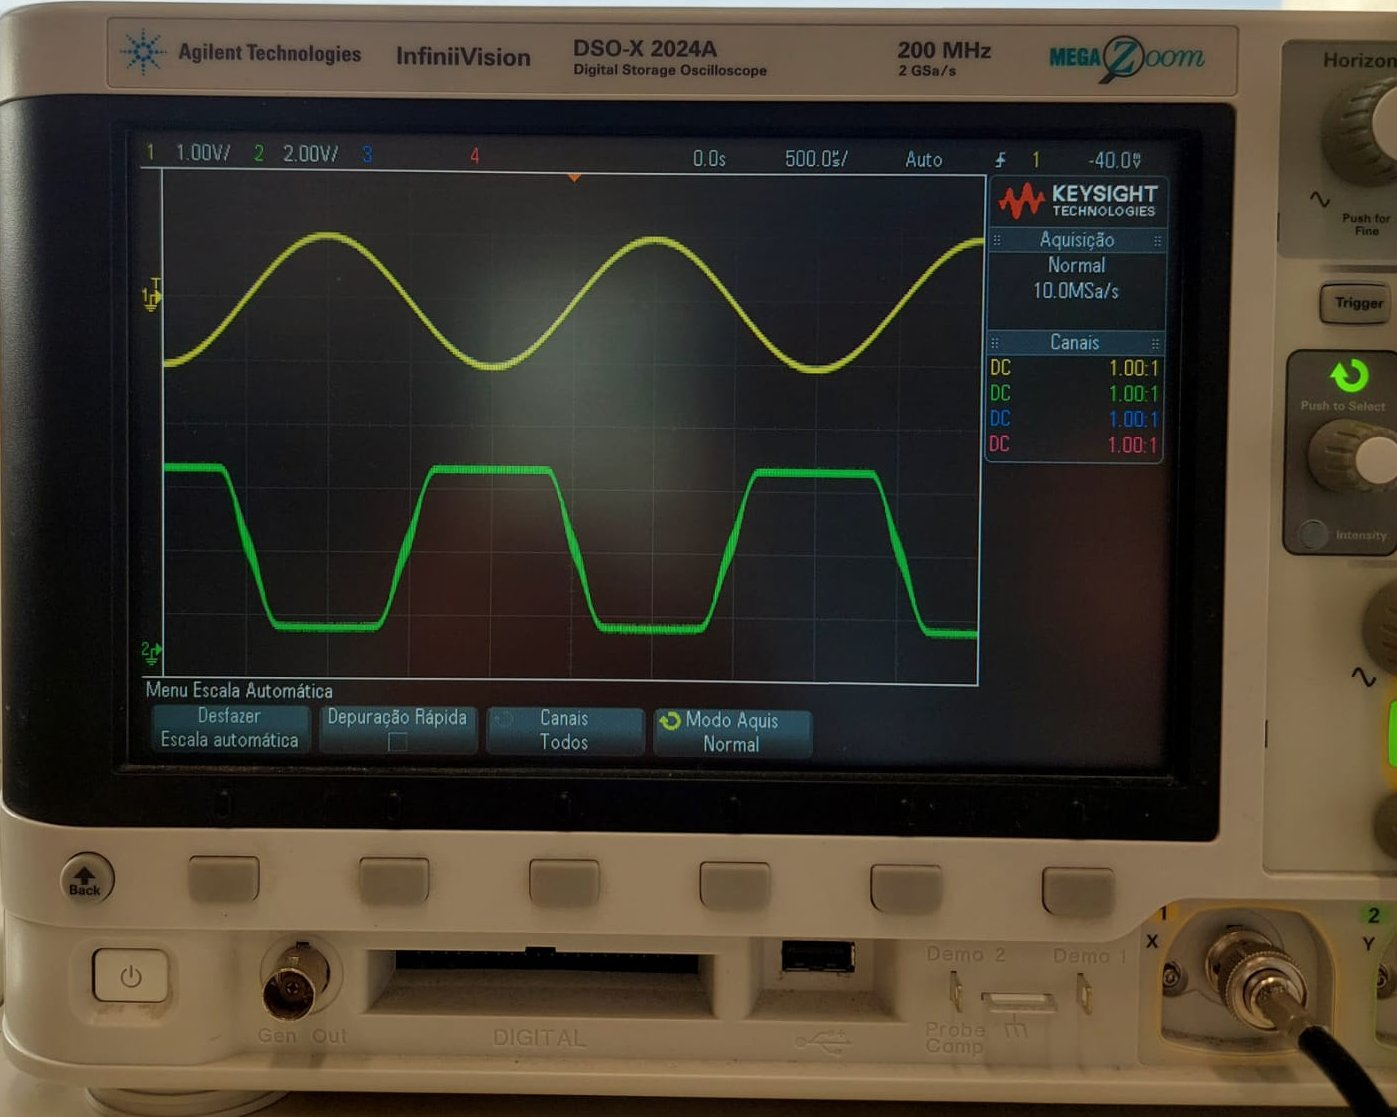
\includegraphics[width=0.9\textwidth]{5.2-1.jpeg} % first figure itself
                                                \caption{A amarelo v$_1$, a verde v$_{o1}$}
                                          \end{minipage}\hfill
                                          \begin{minipage}{0.45\textwidth}
                                                  \centering
                                                  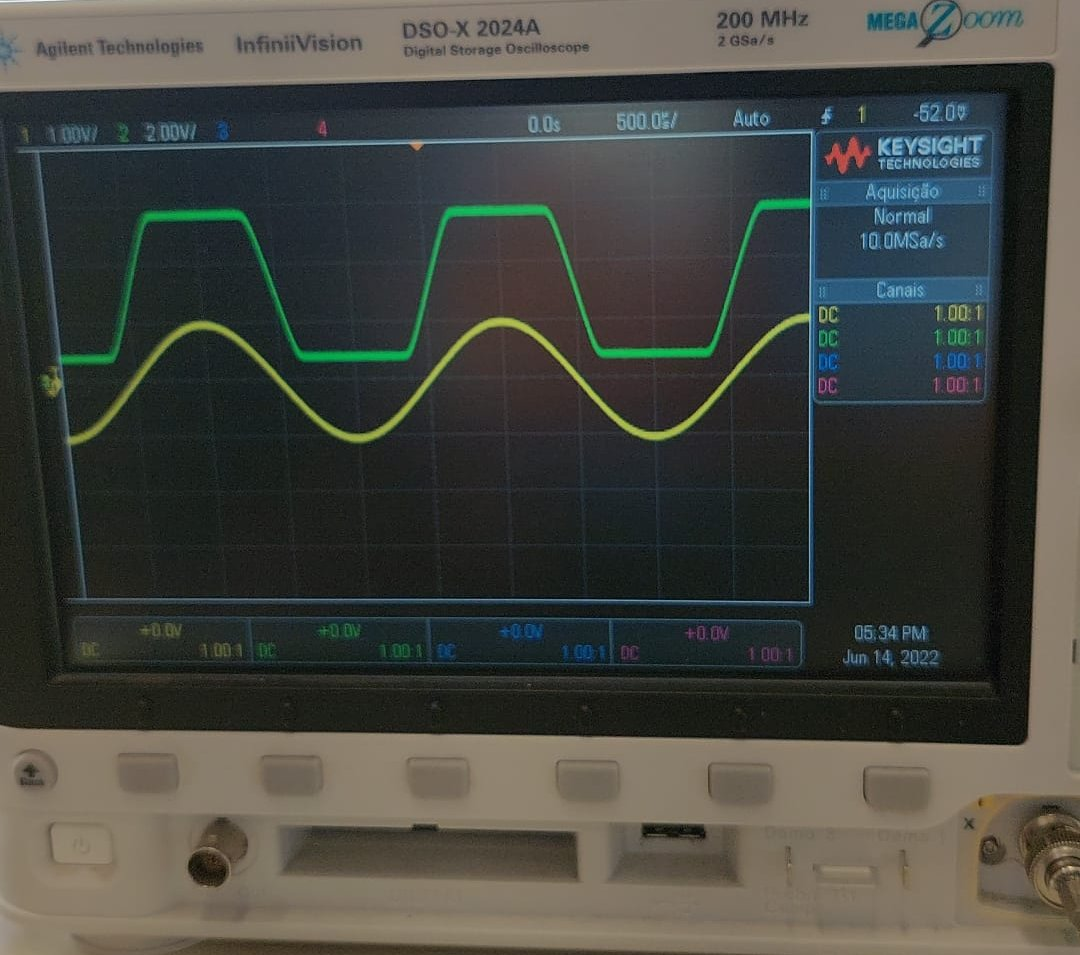
\includegraphics[width=0.9\textwidth]{5.2-2.jpeg} % second figure itself
                                               \caption{A amarelo v$_1$ a verde v$_{o2}$}
                                                  \end{minipage}
                                  \end{figure}
			\begin{figure}[H]
                                            \centering
                                            \begin{minipage}{0.45\textwidth}
                                                    \centering
                                                    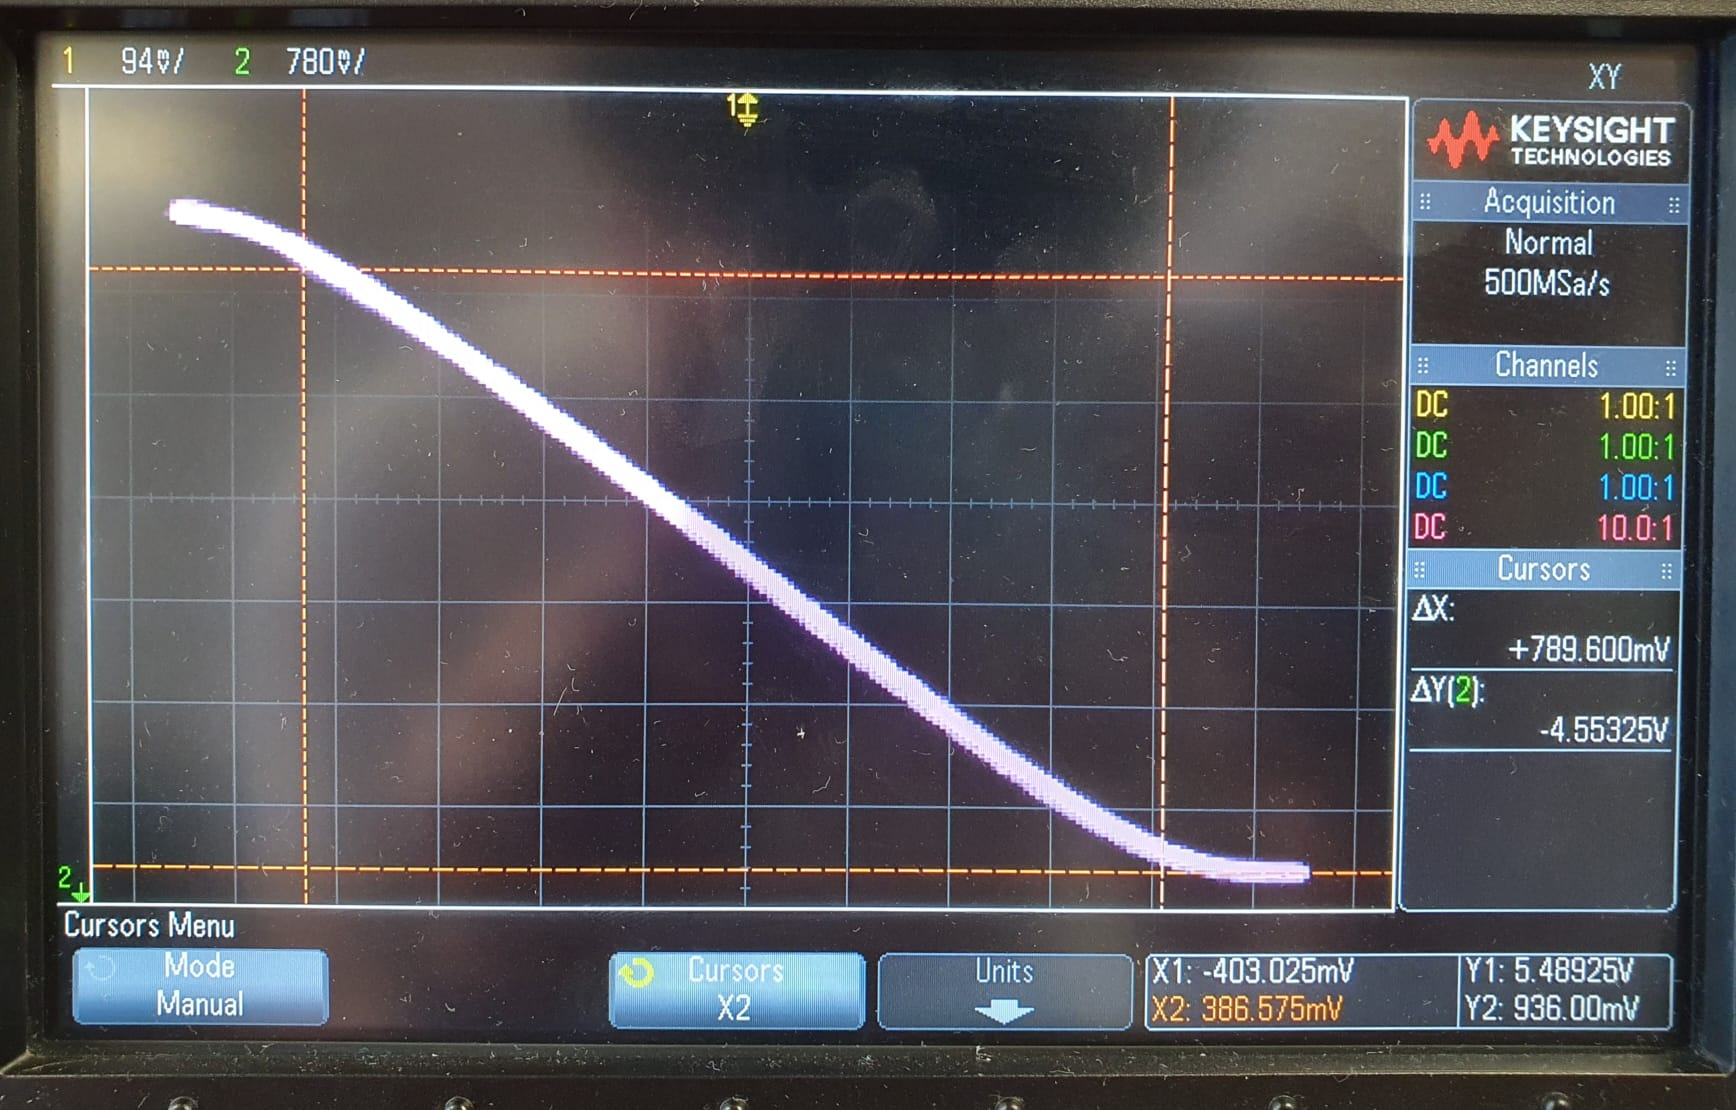
\includegraphics[width=0.9\textwidth]{5.2-4.jpeg} % first figu  re itself
                                                  \caption{V$_{o1}$ em modo X-Y}
                                            \end{minipage}\hfill
                                            \begin{minipage}{0.45\textwidth}
                                                    \centering
                                                    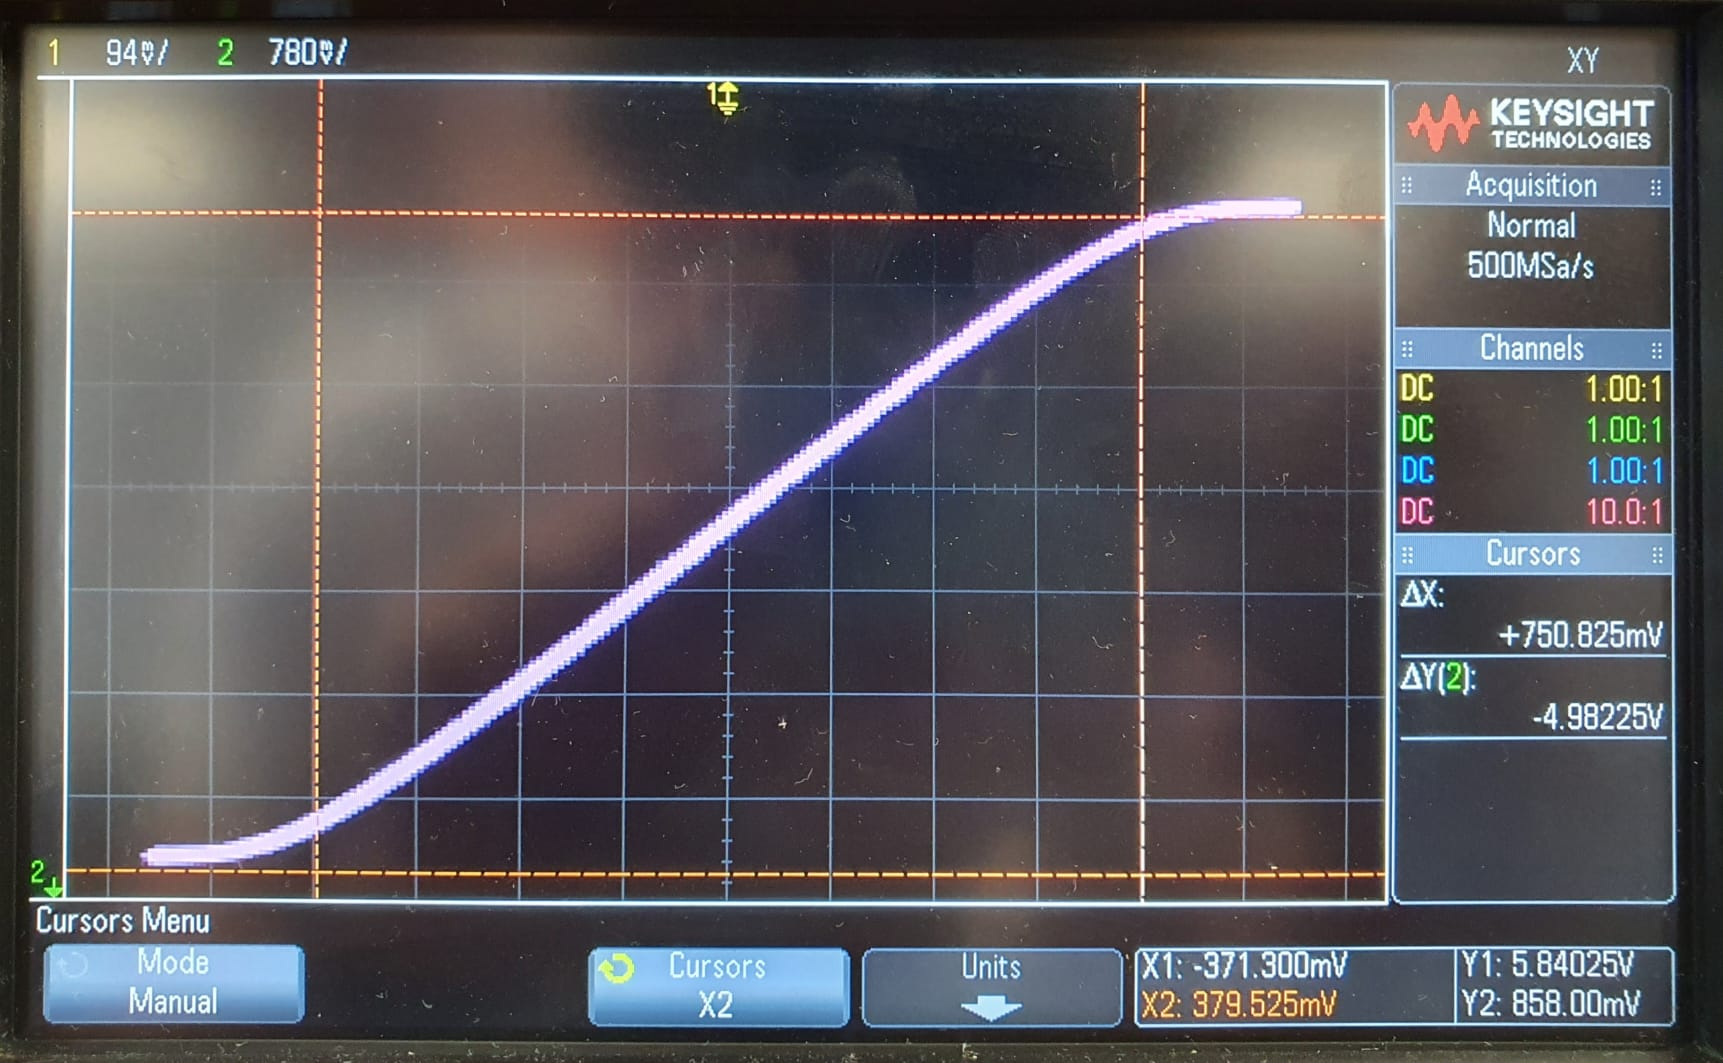
\includegraphics[width=0.9\textwidth]{5.2-3.jpeg} % second fig  ure itself
                                                 \caption{V$_{o2}$ em modo X-Y}
                                                    \end{minipage}
                                    \end{figure}
				    Com os ganhos Ad1 e Ad2 iguais aos declives ($\Delta Y$) respectivos
	\newpage
	 \section{Questão 5.3}
	 Distinto do que ocorre na situação anterior, em modo AC não ocorre saturação, permitindo assim uma fácil determinação dos ganhos pela análise visual das amplitudes \newline
	 \begin{figure}[H]
                                          \centering
                                          \begin{minipage}{0.45\textwidth}
                                                  \centering
                                                  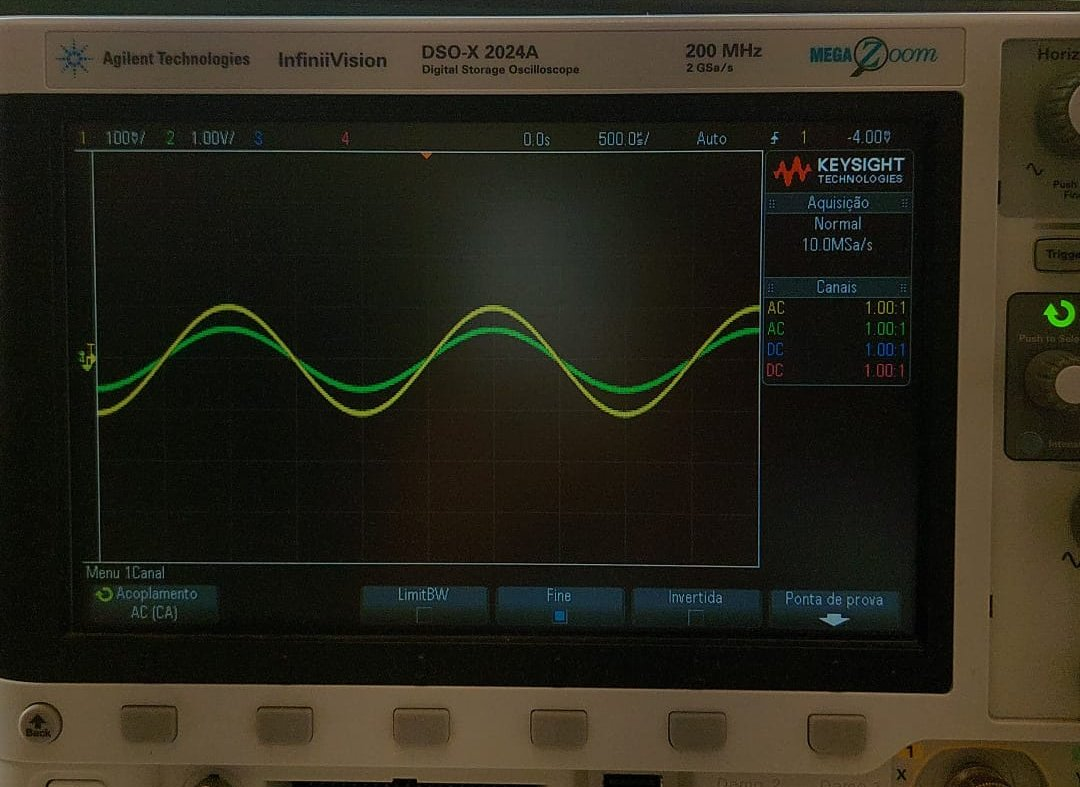
\includegraphics[width=0.9\textwidth]{5.3-4.jpeg} % first figure itself
                                                \caption{}
                                          \end{minipage}\hfill
                                          \begin{minipage}{0.45\textwidth}
                                                  \centering
                                                  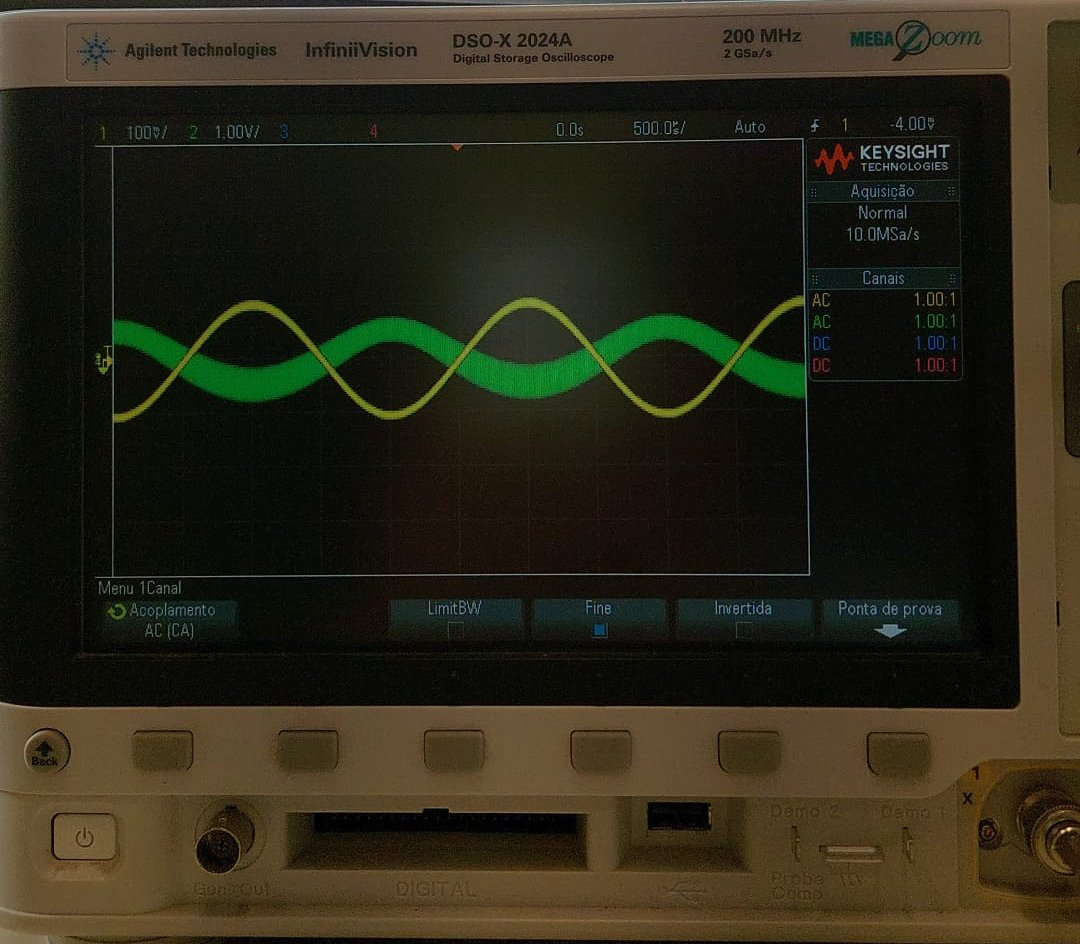
\includegraphics[width=0.9\textwidth]{5.3-3.jpeg} % second figure itself
                                               \caption{}
                                                  \end{minipage}
                                  \end{figure}
				 \begin{figure}[H]
                          \centering
                          \captionsetup{justification=centering}
                          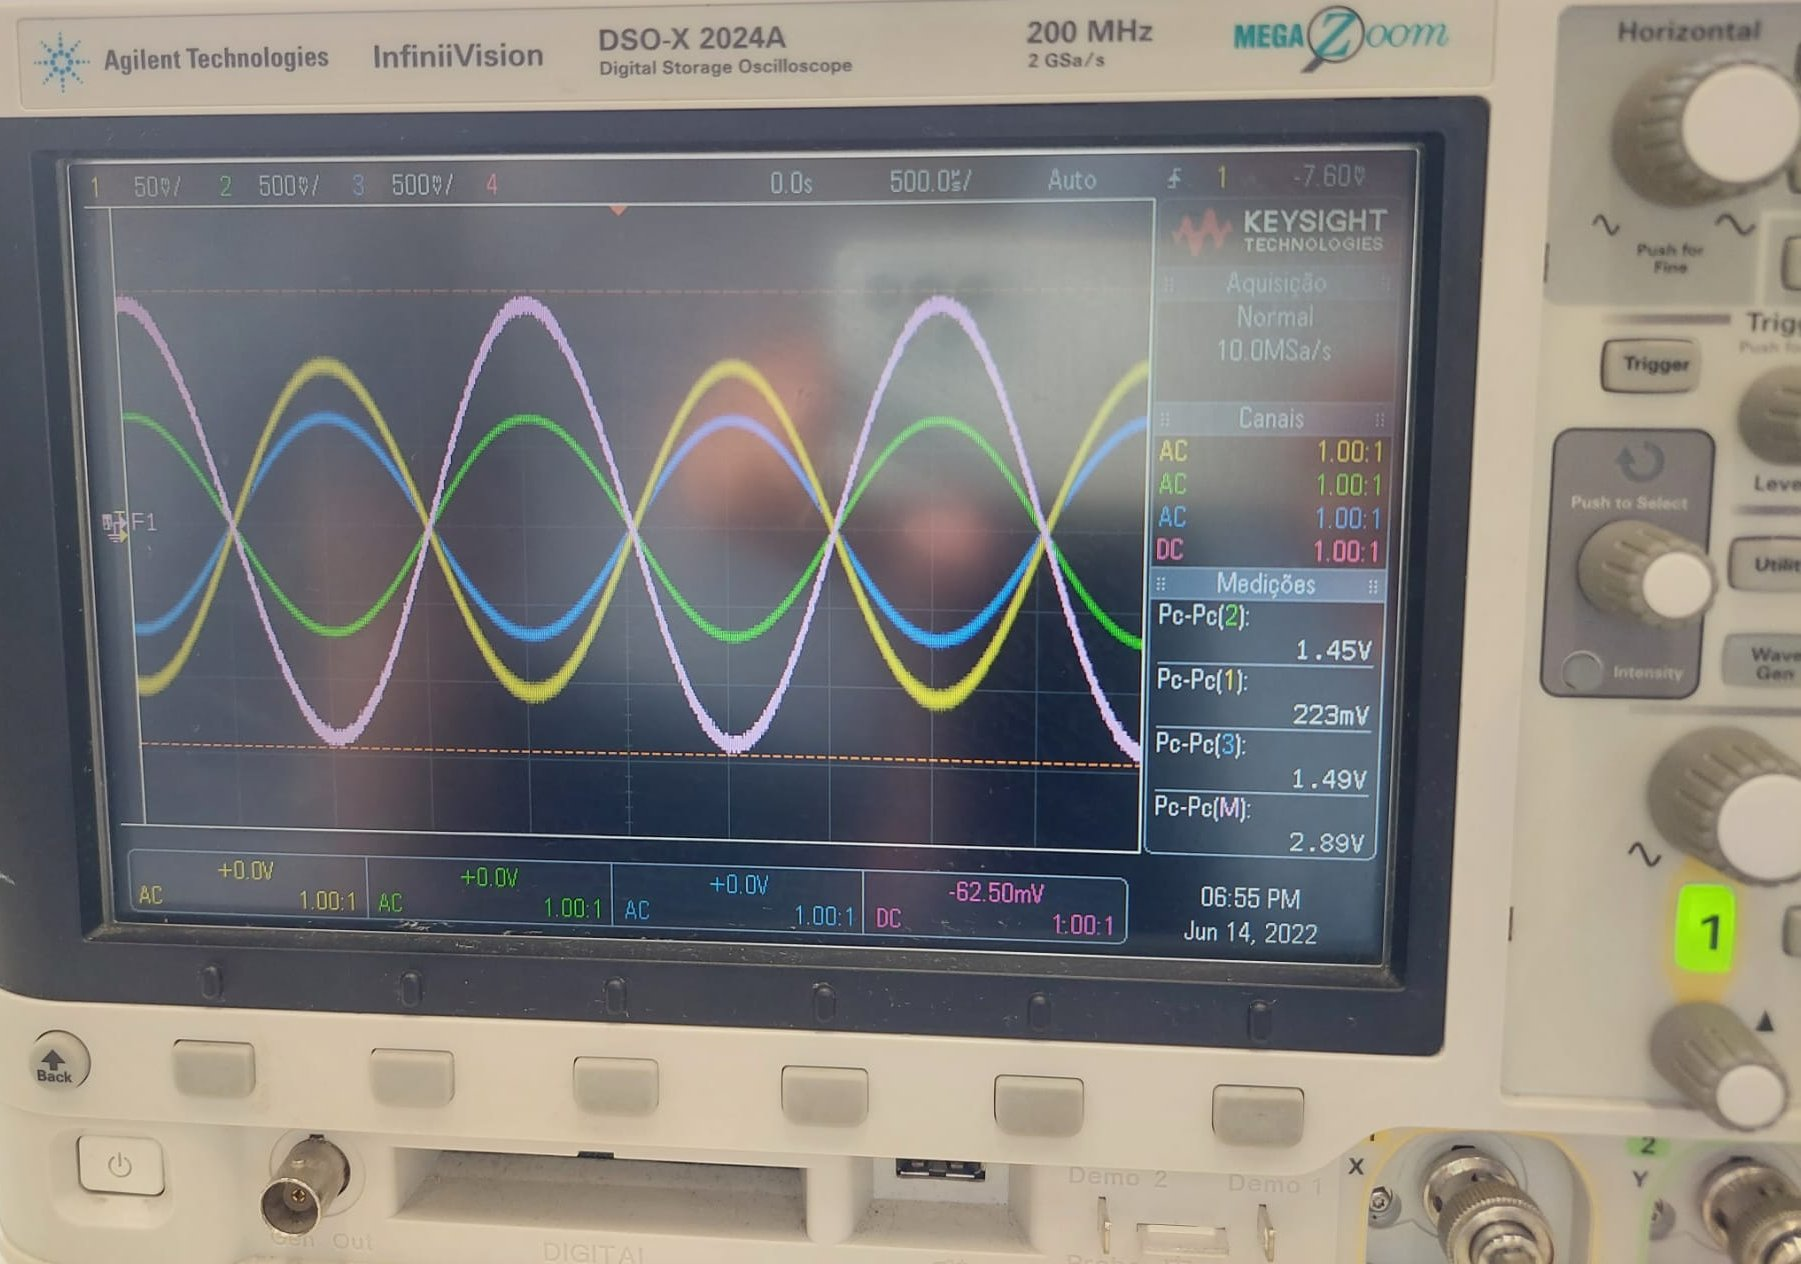
\includegraphics[scale=0.15\textscale]{5.3-1.jpeg}
                          \caption{V1 (a verde), vo1(a amarelo), vo2 (a azul ) e vo12 (a rosa)}
                  \end{figure}
		  Obtém-se então os ganhos Ad1, Ad2 e Ad:
\begin{center}
			    \begin{equation}
				    Ad1=\frac{vo1}{v1}=0.154
				\end{equation}
			\begin{equation}
			Ad2=\frac{vo2}{v1}=1.027
			\end{equation}
			\begin{equation}
			Ad=\frac{vo12}{v1}=1.993
			\end{equation}

		\end{center}

	\newpage
	\section{Conclusões}
		O trabalho correu como o esperado, assim como os resultados que foram semelhantes á analise teórica, tanto os simulados como os experimentais.\newline
A chave para o funcionamento do par diferencial está relacionada com a sua simetria. No entanto, um circuito real não é ideal, pelo que notamos pequenas disparidades em alguns dos valores medidos.\newline
Por fim, é interessante o facto de haver ruído, porque naturalmente um par diferencial seria menos suscetível a ruído, no entanto, neste caso o ruído está todo associado a apenas uma das entradas, não sendo anulado na diferenciabilidade do par, logo não se nota esta qualidade do par diferencial.
\end{document}
